% !TeX program = lualatex
% !BIB program = biber
% Lualatex is important to render TTF fonts; with pdflatex it's just the regular one
% ratio 16:9 -- https://tex.stackexchange.com/questions/14336/

% compile two versions, inspired by https://tex.stackexchange.com/a/1501
% use the script "compile-pdf.sh"
\newif\ifhandout
% if flags.tex does not exist, create an empty file to be able to compile in TeXstudio
\input{flags}

\ifhandout
\documentclass[12pt,aspectratio=169,handout]{beamer}
\else
\documentclass[12pt,aspectratio=169]{beamer}
\fi



% TODO change "leftfootertext" to your liking
\newcommand{\leftfootertext}{\insertsubtitle}  % just the \title{} text by default
%\newcommand{\leftfootertext}{RNNs and encoder-decoder architectures}  % Your name, for instance


% ------- RUB specifics ----------
% adjust for 16:9
% https://tex.stackexchange.com/questions/354022/modifying-the-margins-of-all-slides-in-beamer
\setbeamersize{text margin left=0.3cm,text margin right=4.5cm} 


% use Metropolis as the basis theme
\usetheme[subsectionpage=progressbar]{metropolis}
% blocks with background globally
\metroset{block=fill}


\usepackage{fontspec}
% RUB fonts need to be installed
% 'UprightFont = * Light' makes sure that the base font is RubFlama Light, which looks
% lighter than RubFlama Regular (would be too thick for slides)
\setsansfont[Scale=MatchLowercase, UprightFont = * Light, BoldFont = * Bold]{RubFlama}
%\setsansfont{Arial} % Open source alternative if you don't have RubFlama

% RUB color scheme
% Dark blue: 0; 53; 96; #003560
\definecolor{RUBDarkBlue}{RGB}{0, 53, 96}

% Light yellow (table fill, etc.); 238; 250; 196; #EEFAC4
\definecolor{RUBLightYellow}{RGB}{238, 250, 196}

%Light green: 141; 174; 16
\definecolor{RUBLightGreen}{RGB}{141, 174, 16}


\setbeamercolor{titlelike}{fg=RUBDarkBlue}
\setbeamercolor{subtitle}{fg=RUBLightGreen}
\setbeamercolor{separation line}{fg=RUBLightGreen}
\setbeamercolor{frametitle}{bg=white, fg=RUBDarkBlue}

% horizontal line on title page and sections
\setbeamercolor{alerted text}{fg=RUBLightGreen}


% Adjust footer bottom (too large by default)
\setbeamertemplate{footline}{%
  \begin{beamercolorbox}[wd=\textwidth, sep=2ex]{footline}%
    \usebeamerfont{page number in head/foot}%
    \usebeamertemplate*{frame footer}
    \hfill%
    \usebeamertemplate*{frame numbering}
  \end{beamercolorbox}%
}


% Lab name, numbering, etc. in footer
\setbeamertemplate{frame numbering}{TrustHLT --- Prof.\ Dr.\ Ivan Habernal \hspace*{1ex} \includegraphics[width=7em]{img/rub-logo.pdf}\hspace*{1ex}}

\setbeamertemplate{frame footer}{\hspace*{1ex}\insertframenumber \hspace*{2ex} \leftfootertext}

% adjust the background to be completely white
\setbeamercolor{background canvas}{bg=white}

% logos on the title page
\titlegraphic{%
	\begin{picture}(0,0)
		\put(435,0){\makebox(0,0)[rt]{\includegraphics[width=7em]{img/rub-logo.pdf}}}
		\put(435,-170){\makebox(0,0)[rt]{\includegraphics[width=4em]{img/logo-trusthlt.pdf}}}
		\put(435,-196){\makebox(0,0)[rt]{\includegraphics[width=9em]{img/logo-rctrust.pdf}}}
	\end{picture}%
}


% show TOC at every section start
\AtBeginSection{
	\frame{
		\vspace{2em}
		\sectionpage
		\hspace*{2.2em}\begin{minipage}{10cm}
			\tableofcontents[currentsection]
		\end{minipage}
	}
}

% TOC without subsection
\setcounter{tocdepth}{1} % only-- part,chapters,sections 

% bullet points: rectangles
\useinnertheme{rectangles}
\setbeamercolor{itemize item}{fg=RUBLightGreen}
\setbeamercolor{itemize subitem}{fg=RUBLightGreen}
% enumerate: blue background for better readability
\setbeamercolor{item projected}{bg=RUBDarkBlue}

% make boxes (example, block, etc.) background lighter for readability
\setbeamercolor{block title}{%
	use=normal text,
	fg=normal text.fg,
	bg=normal text.bg!90!fg % lighter background in block title
}
\setbeamercolor{block body}{
	use={block title, normal text},
	bg=block title.bg!30!normal text.bg % lighter background in block body
}


% RUB colors in blocks
\setbeamercolor{block title alerted}{%
	use={block title, alerted text},
	bg=RUBDarkBlue,
	%fg=RUBLightYellow % looks bad
	fg=white % better contrast
}

\setbeamercolor{block title example}{%
	use={block title, example text},
	fg=RUBLightGreen
}


% ------- end of RUB specifics ----------

% all itemize with pause by default
%\beamerdefaultoverlayspecification{<+->}


% typeset mathematics on serif
\usefonttheme[onlymath]{serif}

% better bibliography using biber as backend
\usepackage[natbib=true,backend=biber,style=authoryear-icomp,maxbibnames=30,maxcitenames=9,uniquelist=false,giveninits=true,doi=false,url=false,dashed=false,isbn=false]{biblatex}
% shared bibliography
\addbibresource{../../nlpwdl-bibliography.bib}
% disable "ibid" for repeated citations
\boolfalse{citetracker}



\usepackage{xspace}


% for derivatives, https://tex.stackexchange.com/a/412442
\usepackage{physics}

\usepackage{tikz}
\usetikzlibrary{matrix, positioning}
\usetikzlibrary{angles,quotes} % for angles
\usetikzlibrary{backgrounds} % background
\usetikzlibrary{decorations.pathreplacing} % curly braces
\usetikzlibrary{calligraphy}
\usetikzlibrary{calc} % for neural nets

% for plotting functions
\usepackage{pgfplots}
\usepgfplotslibrary{dateplot}

% sub-figures
\usepackage{caption}
\usepackage{subcaption}

% book tabs
\usepackage{booktabs}


% argmin, argmax
\usepackage{amsmath}
\DeclareMathOperator*{\argmax}{arg\!\max}
\DeclareMathOperator*{\argmin}{arg\!\min}
% softmax
\DeclareMathOperator*{\softmax}{soft\!\max}
% Mask
\DeclareMathOperator*{\mask}{mask}

% bold math
\usepackage{bm}

% for \mathclap
\usepackage{mathtools}

% algorithms
\usepackage[noend]{algpseudocode}


% for neurons and layers in tikz
\tikzset{
	neuron/.style={draw, rectangle, inner sep=2pt, minimum width=0.75cm, fill=blue!20},
	param/.style={draw, rectangle, inner sep=2pt, minimum width=0.75cm, fill=green!20},
	constant/.style={draw, rectangle, inner sep=2pt, minimum width=0.75cm, fill=black!15},
	% for citation nodes right top
	ref/.style={anchor = north east, text width=7.8cm, yshift=-1.3cm, xshift=-0.2cm, scale=0.5},
	state/.style={rectangle, inner sep=2pt, minimum width=0.75cm, fill=black!5},
}

% added in lecture 10
\tikzset{
	mtx/.style={
		matrix of math nodes,
		left delimiter={[}, right delimiter={]}
	},
	hlt/.style={opacity=0.1, line width=4 mm, line cap=round},
	hltr/.style={opacity=0.5, rounded corners=2pt, inner sep=-1pt}
}

% for strike-through text (added in Lecture 06)
\usepackage[normalem]{ulem}

% added in Lecture 7
% RNN
\DeclareMathOperator*{\rnn}{RNN}
% RNN star
\DeclareMathOperator*{\rnnstar}{RNN^{*}}
% bi-RNN
\DeclareMathOperator*{\birnn}{biRNN}


% added in Lecture 9
\usetikzlibrary{fit} % for hightligting by calling "fit"

% algorithms
\usepackage[noend]{algpseudocode}



\title{Natural Language Processing with Deep Learning}
\subtitle{Lecture 6 --- Word embeddings and RNNs}
\date{November 20, 2025}
\author{Prof.\ Dr.\ Ivan Habernal}
\institute{
\texttt{www.trusthlt.org} \\
Trustworthy Human Language Technologies Group (TrustHLT) \\
Ruhr University Bochum \& Research Center Trustworthy Data Science and Security}



\begin{document}

\maketitle



\section{Last lecture}

\begin{frame}{Learned word representations as a by-product}
\vspace{-1em}
\begin{figure}
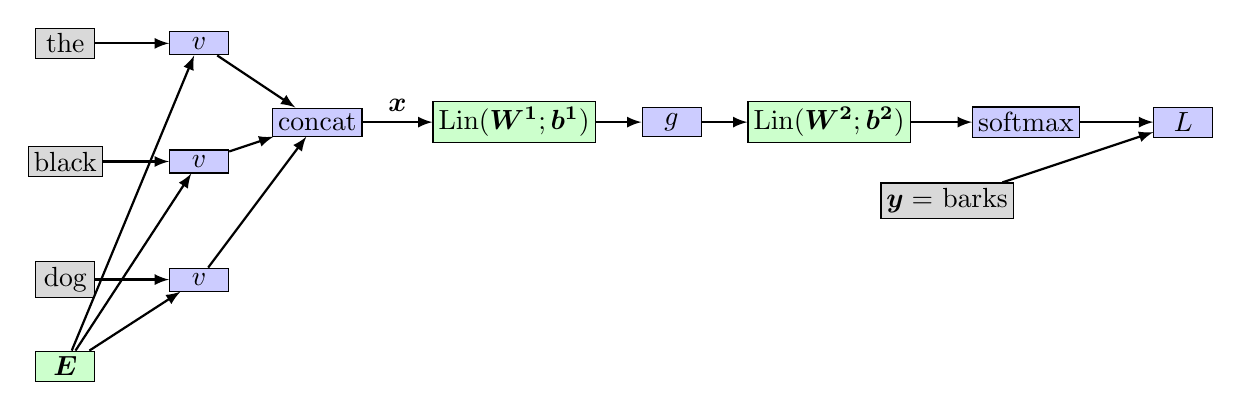
\begin{tikzpicture}	
	%\node (a1) [draw, circle, inner sep=0pt, minimum width=0.75cm, fill=green!20] {$a_1$};
	
	\node (the) [constant] {the};
	\node (black) [constant, below of=the, yshift=-0.5cm]{black};
	\node (dog) [constant, below of=black, yshift=-0.5cm]{dog};
	\node (e) [param, below of=dog, yshift=-0.1cm] {$\bm{E}$};
	
	\node (lookup1) [neuron, right of=the, xshift=0.7cm] {$v$};
	\node (lookup2) [neuron, below of=lookup1, yshift=-0.5cm] {$v$};
	\node (lookup3) [neuron, below of=lookup2, yshift=-0.5cm] {$v$};			
	\node (concat) [neuron, right of=lookup1, xshift=0.5cm, yshift=-1cm] {concat};
	
	
	%			\node (x) [constant, right of=concat, xshift=1cm] {$\bm{x}$};
	\node (f1) [param, right of=concat, xshift=1.5cm] {Lin$(\bm{W^1};\bm{b^1})$};
	
	\node (g) [neuron, right of=f1, xshift=1cm] {$g$};
	\node (f2) [param, right of=g, xshift=1cm] {Lin$(\bm{W^2};\bm{b^2})$};
	
	\node (softmax) [neuron, right of=f2, xshift=1.5cm] {$\softmax$};
	
	\node (l) [neuron, right of=softmax, xshift=1cm] {$L$};
	\node (y) [constant, below of=f2, xshift=1.5cm] {$\bm{y} =$ barks};
	
	\begin{scope}[thick, black, ->, >=latex]
		\draw (the) -- (lookup1);
		\draw (black) -- (lookup2);
		\draw (dog) -- (lookup3);
		\draw (e) -- (lookup1);
		\draw (e) -- (lookup2);
		\draw (e) -- (lookup3);
		
		\draw (lookup1) -- (concat);
		\draw (lookup2) -- (concat);
		\draw (lookup3) -- (concat);								
		
		\draw (concat) -- (f1) node [midway, above] {$\bm{x}$};
		\draw (f1) -- (g);
		\draw (g) -- (f2);
		\draw (f2) -- (softmax);
		\draw (softmax) -- (l);
		\draw (y) -- (l);
	\end{scope}	
\end{tikzpicture}
\end{figure}
	
Each row of $\bm{E}$ learns a word representation
	
	
\end{frame}

\section{Learning word embeddings}





\subsection{Distributional hypothesis}

\begin{frame}{Recall: One-hot encoding of words}
	
Major drawbacks?

\begin{itemize}
	\item No `semantic' similarity, all words are equally `similar'
\end{itemize}

\begin{block}{Example (see Lecture 3 for more)}
	$
	V = \begin{pmatrix}
		\text{a}_1 & \text{abandon}_2 & \ldots & \text{zone}_{2,999} & \text{zoo}_{3,000}
	\end{pmatrix}
	$
	
	\bigskip
	$
	\begin{aligned}
		\text{nice} &= 
		\begin{pmatrix}
			0_1 & \ldots & 1_{1,852} & \ldots & 0_{2,999} & 0_{3,000}
		\end{pmatrix} \\
		\text{pleasant} &= 
		\begin{pmatrix}
			0_1 & \ldots & 1_{2,012} & \ldots & 0_{2,999} & 0_{3,000}
		\end{pmatrix} \\
		\text{horrible} &= 
		\begin{pmatrix}
			0_1 & \ldots & 1_{696} & \ldots & 0_{2,999} & 0_{3,000}
		\end{pmatrix} \\
	\end{aligned}
	$
	
\end{block}


\end{frame}

\begin{frame}{Distributional hypothesis}

The distributional hypothesis stating that \emph{words are similar if they appear in similar contexts}

\begin{example}
Intuitively, when we encounter a sentence with an unknown word such as the word \textbf{wampinuk} in

\pause
\emph{Marco saw a hairy little \textbf{wampinuk} crouching behind a tree}

We infer the meaning of the word based on the context in which it occurs
\end{example}

\end{frame}


\begin{frame}{From neural language models to training word embeddings}
(Neural) language model's goal: Predict probability distribution over $|V|$ for the next word conditioned on the previous words

\begin{itemize}
	\item Side product: Can learn useful word embeddings
\end{itemize}

\pause
What if we don't need probability distribution but just want to learn word embeddings?
\begin{itemize}
	\item We can relax our Markov assumption of `look at $k$ previous words only'
	\item We can get rid of the costly normalization in softmax
\end{itemize}
	
\end{frame}

\begin{frame}{Simplification 1: Ditch the Markov property --- look into the future!}
	\vspace{-1em}
%	$$	f(\bm{x}) = g \left(	\bm{x} \bm{W^1} + \bm{b^1}	\right)	\bm{W^2} + \bm{b^2}	$$
\begin{figure}
	\begin{tikzpicture}	
		%\node (a1) [draw, circle, inner sep=0pt, minimum width=0.75cm, fill=green!20] {$a_1$};
		
		\node (the) [constant] {the};
		\node (black) [constant, below of=the, yshift=-0.5cm, opacity=0.2]{black};
		\node (dog) [constant, below of=black, yshift=-0.5cm]{dog};
		\node (e) [param, below of=dog, yshift=-0.1cm] {$\bm{E}$};
		
		\node (lookup1) [neuron, right of=the, xshift=0.7cm] {$v$};
%		\node (lookup2) [neuron, below of=lookup1, yshift=-0.5cm] {$v$};
		\node (lookup3) [neuron, below of=lookup2, yshift=-0.5cm] {$v$};			
		\node (concat) [neuron, right of=lookup1, xshift=0.5cm, yshift=-1cm] {concat};
		
		
		%			\node (x) [constant, right of=concat, xshift=1cm] {$\bm{x}$};
		\node (f1) [param, right of=concat, xshift=1.5cm] {Lin$(\bm{W^1};\bm{b^1})$};
		
		\node (g) [neuron, right of=f1, xshift=1cm] {$g$};
		\node (f2) [param, right of=g, xshift=1cm] {Lin$(\bm{W^2};\bm{b^2})$};
		
		\node (softmax) [neuron, right of=f2, xshift=1.5cm] {$\softmax$};
		
		\node (l) [neuron, right of=softmax, xshift=1cm] {$L$};
		\node (y) [constant, below of=f2, xshift=1.5cm] {$\bm{y} =$ black};
		
		\begin{scope}[thick, black, ->, >=latex]
			\draw (the) -- (lookup1);
%			\draw (black) -- (lookup2);
			\draw (dog) -- (lookup3);
			\draw (e) -- (lookup1);
%			\draw (e) -- (lookup2);
			\draw (e) -- (lookup3);
			
			\draw (lookup1) -- (concat);
%			\draw (lookup2) -- (concat);
			\draw (lookup3) -- (concat);								
			
			\draw (concat) -- (f1) node [midway, above] {$\bm{x}$};
			\draw (f1) -- (g);
			\draw (g) -- (f2);
			\draw (f2) -- (softmax);
			\draw (softmax) -- (l);
			\draw (y) -- (l);
		\end{scope}	
	\end{tikzpicture}
\end{figure}	

For example, instead of modeling $\Pr(w_3 | w_1, w_2, \boxdot)$, we model $\Pr(w_2 | w_1,  \boxdot, w_3)$

\end{frame}

\begin{frame}{Simplification 2: Give up the costly probability distribution}

Instead of predicting probability distribution over the entire vocabulary, we just want to predict some score of \textbf{context} and \textbf{target word}

What could such a score be?

\pause

\begin{itemize}
	\item Prefer words in their true contexts (high score)
	\pause
	\item Penalize words in their `untrue' contexts (low score)
\end{itemize}

\end{frame}


\begin{frame}{Negative sampling}
	
Instead of predicting probability distribution for the target word, we \textbf{create an artificial binary task} by choosing either the correct or a random incorrect target word \pause
$$
y = 
 \begin{cases}
	1  & \quad \text{if } (w, c_{1:k}) \text{ is a positive example from the corpus}\\
	0  & \quad \text{if } (w', c_{1:k}) \text{ is a negative example from the corpus}\\
\end{cases}
$$

\pause
Which distribution for sampling $w'$ from $V$?
\begin{itemize}
	\item Corpus-based frequency: $\frac{\#(v)}{\sum_{v' \in V} \#(v')}$ (pr.\ of each word $v$)
	\item Re-weighted: $\frac{\#(v)^{0.75}}{\sum_{v' \in V} \#(v')^{0.75}}$ (more weight on less frequent words done in word2vec)
\end{itemize}
	
\end{frame}

\begin{frame}{Turn the problem into binary classification (positive example)}


\begin{figure}
	\begin{tikzpicture}	
		%\node (a1) [draw, circle, inner sep=0pt, minimum width=0.75cm, fill=green!20] {$a_1$};
		
		\node (the) [constant] {the};
		
		\node (black) [constant, below of=the, yshift=-0.5cm, opacity=0.5]{black};

		\node (dog) [constant, below of=black, yshift=-0.5cm]{dog};
		\node (e) [param, below of=dog, yshift=-0.1cm] {$\bm{E}$};
		
		\node (lookup1) [neuron, right of=the, xshift=0.7cm] {$v$};
		\node (lookup2) [neuron, below of=lookup1, yshift=-0.5cm] {$v$};
		\node (lookup3) [neuron, below of=lookup2, yshift=-0.5cm] {$v$};			
		\node (concat) [neuron, right of=lookup1, xshift=1cm, yshift=-1cm] {model the context};
		
		
		%			\node (x) [constant, right of=concat, xshift=1cm] {$\bm{x}$};
		\node (f1) [neuron, right of=concat, xshift=1.5cm, yshift=-1cm] {somehow combine};
		
%		\node (g) [neuron, right of=f1, xshift=1cm] {$g$};
		\node (f2) [param, right of=g, xshift=0cm, yshift=1cm] {some hidden layers};
		
		\node (softmax) [neuron, right of=f2, xshift=1.5cm, yshift=-1cm] {$\sigma$};
		
		\node (l) [neuron, right of=softmax, xshift=1cm] {$L$};
		\node (y) [constant, below of=softmax, xshift=1.5cm] {$y = 1$};
		
		\begin{scope}[thick, black, ->, >=latex]
			\draw (the) -- (lookup1);
			\draw (black) -- (lookup2);
			\draw (dog) -- (lookup3);
			\draw (e) -- (lookup1);
			\draw (e) -- (lookup2);
			\draw (e) -- (lookup3);
			
			\draw (lookup1) -- (concat);
			\draw (lookup2) -- (f1);
			\draw (lookup3) -- (concat);								
			
			\draw (concat) -- (f1);
%			\draw (f1) -- (g);
			\draw (f1) -- (f2);
			\draw (f2) -- (softmax);
			\draw (softmax) -- (l);
			\draw (y) -- (l);
		\end{scope}	
	\end{tikzpicture}
\end{figure}	
	
\end{frame}

\begin{frame}{Turn the problem into binary classification (negative example)}
	
	
	\begin{figure}
		\begin{tikzpicture}	
			%\node (a1) [draw, circle, inner sep=0pt, minimum width=0.75cm, fill=green!20] {$a_1$};
			
			\node (the) [constant] {the};
			
			\node (black) [constant, below of=the, yshift=-0.5cm, opacity=0.5]{with};
			
			\node (dog) [constant, below of=black, yshift=-0.5cm]{dog};
			\node (e) [param, below of=dog, yshift=-0.1cm] {$\bm{E}$};
			
			\node (lookup1) [neuron, right of=the, xshift=0.7cm] {$v$};
			\node (lookup2) [neuron, below of=lookup1, yshift=-0.5cm] {$v$};
			\node (lookup3) [neuron, below of=lookup2, yshift=-0.5cm] {$v$};			
			\node (concat) [neuron, right of=lookup1, xshift=1cm, yshift=-1cm] {model the context};
			
			
			%			\node (x) [constant, right of=concat, xshift=1cm] {$\bm{x}$};
			\node (f1) [neuron, right of=concat, xshift=1.5cm, yshift=-1cm] {somehow combine};
			
			%		\node (g) [neuron, right of=f1, xshift=1cm] {$g$};
			\node (f2) [param, right of=g, xshift=0cm, yshift=1cm] {some hidden layers};
			
			\node (softmax) [neuron, right of=f2, xshift=1.5cm, yshift=-1cm] {$\sigma$};
			
			\node (l) [neuron, right of=softmax, xshift=1cm] {$L$};
			\node (y) [constant, below of=softmax, xshift=1.5cm] {$y = 0$};
			
			\begin{scope}[thick, black, ->, >=latex]
				\draw (the) -- (lookup1);
				\draw (black) -- (lookup2);
				\draw (dog) -- (lookup3);
				\draw (e) -- (lookup1);
				\draw (e) -- (lookup2);
				\draw (e) -- (lookup3);
				
				\draw (lookup1) -- (concat);
				\draw (lookup2) -- (f1);
				\draw (lookup3) -- (concat);								
				
				\draw (concat) -- (f1);
				%			\draw (f1) -- (g);
				\draw (f1) -- (f2);
				\draw (f2) -- (softmax);
				\draw (softmax) -- (l);
				\draw (y) -- (l);
			\end{scope}	
		\end{tikzpicture}
	\end{figure}	
	
\end{frame}



\section{word2vec}

\begin{frame}{word2vec}
word2vec simplifies the neural LM by removing the hidden layer (so turning it into a log-linear model!)

\begin{figure}
	\begin{tikzpicture}	
		%\node (a1) [draw, circle, inner sep=0pt, minimum width=0.75cm, fill=green!20] {$a_1$};
		
		\node (the) [constant] {the};
		
		\node (black) [constant, below of=the, yshift=-0.5cm, opacity=0.5]{black};
		
		\node (dog) [constant, below of=black, yshift=-0.5cm]{dog};
		\node (e) [param, below of=dog, yshift=-0.1cm] {$\bm{E}$};
		
		\node (lookup1) [neuron, right of=the, xshift=0.7cm] {$v$};
		\node (lookup2) [neuron, below of=lookup1, yshift=-0.5cm] {$v$};
		\node (lookup3) [neuron, below of=lookup2, yshift=-0.5cm] {$v$};			
		\node (concat) [neuron, right of=lookup1, xshift=1cm, yshift=-1cm] {model the context};
		
		
		%			\node (x) [constant, right of=concat, xshift=1cm] {$\bm{x}$};
		\node (f1) [neuron, right of=concat, xshift=1.5cm, yshift=-1cm] {somehow combine};
		
		%		\node (g) [neuron, right of=f1, xshift=1cm] {$g$};
		\node (f2) [param, right of=g, xshift=0cm, yshift=1cm] {\sout{some hidden layers}};
		
		\node (softmax) [neuron, right of=f2, xshift=1.5cm, yshift=-1cm] {$\sigma$};
		
		\node (l) [neuron, right of=softmax, xshift=1cm] {$L$};
		\node (y) [constant, below of=softmax, xshift=1.5cm] {$y = 1$};
		
		\begin{scope}[thick, black, ->, >=latex]
			\draw (the) -- (lookup1);
			\draw (black) -- (lookup2);
			\draw (dog) -- (lookup3);
			\draw (e) -- (lookup1);
			\draw (e) -- (lookup2);
			\draw (e) -- (lookup3);
			
			\draw (lookup1) -- (concat);
			\draw (lookup2) -- (f1);
			\draw (lookup3) -- (concat);								
			
			\draw (concat) -- (f1);
			%			\draw (f1) -- (g);
%			\draw (f1) -- (f2);
			\draw (f1) -- (softmax);
			\draw (softmax) -- (l);
			\draw (y) -- (l);
		\end{scope}	
	\end{tikzpicture}
\end{figure}	

\end{frame}


\begin{frame}{word2vec --- how to model the context?}
	
\pause

\begin{figure}
	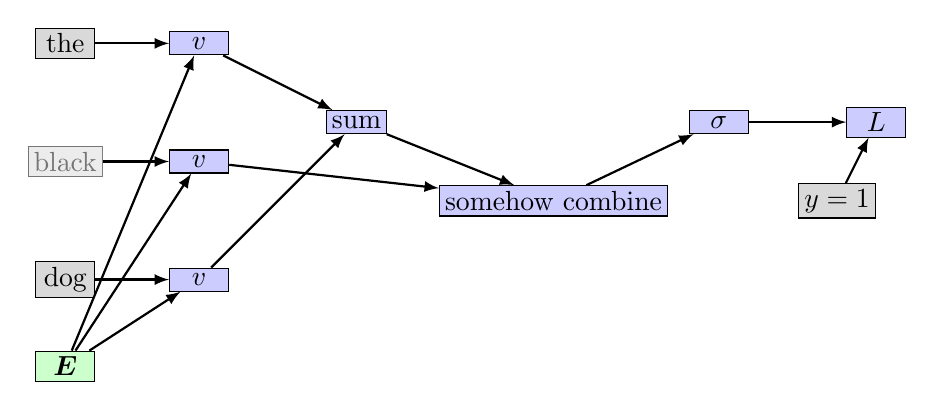
\begin{tikzpicture}	
		%\node (a1) [draw, circle, inner sep=0pt, minimum width=0.75cm, fill=green!20] {$a_1$};
		
		\node (the) [constant] {the};
		
		\node (black) [constant, below of=the, yshift=-0.5cm, opacity=0.5]{black};
		
		\node (dog) [constant, below of=black, yshift=-0.5cm]{dog};
		\node (e) [param, below of=dog, yshift=-0.1cm] {$\bm{E}$};
		
		\node (lookup1) [neuron, right of=the, xshift=0.7cm] {$v$};
		\node (lookup2) [neuron, below of=lookup1, yshift=-0.5cm] {$v$};
		\node (lookup3) [neuron, below of=lookup2, yshift=-0.5cm] {$v$};			
		\node (concat) [neuron, right of=lookup1, xshift=1cm, yshift=-1cm] {sum};
		
		
		%			\node (x) [constant, right of=concat, xshift=1cm] {$\bm{x}$};
		\node (f1) [neuron, right of=concat, xshift=1.5cm, yshift=-1cm] {somehow combine};
		
		%		\node (g) [neuron, right of=f1, xshift=1cm] {$g$};
%		\node (f2) [param, right of=g, xshift=0cm, yshift=1cm] {\sout{something complicated}};
		
		\node (softmax) [neuron, right of=f1, xshift=1.1cm, yshift=1cm] {$\sigma$};
		
		\node (l) [neuron, right of=softmax, xshift=1cm] {$L$};
		\node (y) [constant, below of=softmax, xshift=1.5cm] {$y = 1$};
		
		\begin{scope}[thick, black, ->, >=latex]
			\draw (the) -- (lookup1);
			\draw (black) -- (lookup2);
			\draw (dog) -- (lookup3);
			\draw (e) -- (lookup1);
			\draw (e) -- (lookup2);
			\draw (e) -- (lookup3);
			
			\draw (lookup1) -- (concat);
			\draw (lookup2) -- (f1);
			\draw (lookup3) -- (concat);								
			
			\draw (concat) -- (f1);
			%			\draw (f1) -- (g);
			%			\draw (f1) -- (f2);
			\draw (f1) -- (softmax);
			\draw (softmax) -- (l);
			\draw (y) -- (l);
		\end{scope}	
	\end{tikzpicture}
\end{figure}


%- we have obtained the best performance on the task introduced in the next section by building a log-linear classifier with four future and four history words at the input, where the training criterion is to correctly classify the current (middle) word.

Variant 1: Continuous bag of words (CBOW)
$\bm{c} = \sum_{i = 1}^{k} v(c_i)$


\begin{tikzpicture}[overlay, remember picture] 
	\node at (current page.north east)[ref] {\fullcite{Mikolov.et.al.2013.ICLR} \par};
\end{tikzpicture}


\end{frame}


\begin{frame}{Final CBOW word2vec --- similarity score is the dot product}

%	\vspace{-1em}
	%	$$	f(\bm{x}) = g \left(	\bm{x} \bm{W^1} + \bm{b^1}	\right)	\bm{W^2} + \bm{b^2}	$$
	\begin{figure}
		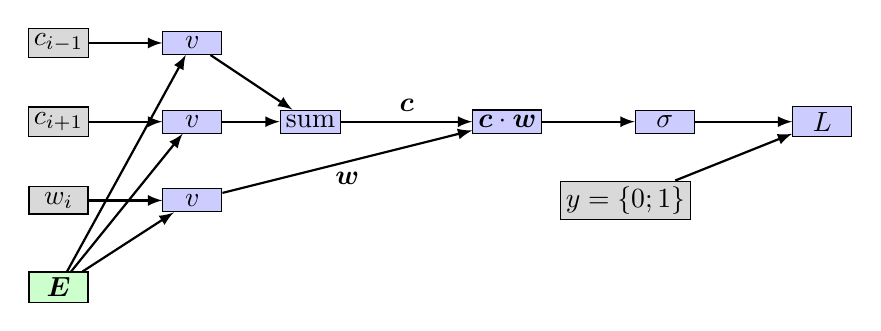
\begin{tikzpicture}	
			%\node (a1) [draw, circle, inner sep=0pt, minimum width=0.75cm, fill=green!20] {$a_1$};
			
			\node (the) [constant] {$c_{i-1}$};
			\node (black) [constant, below of=the, yshift=0cm]{$c_{i+1}$};
			\node (dog) [constant, below of=black, yshift=0cm]{$w_i$};
			\node (e) [param, below of=dog, yshift=-0.1cm] {$\bm{E}$};
			
			\node (lookup1) [neuron, right of=the, xshift=0.7cm] {$v$};
			\node (lookup2) [neuron, below of=lookup1, yshift=0cm] {$v$};
			\node (lookup3) [neuron, below of=lookup2, yshift=0cm] {$v$};			
			\node (concat) [neuron, right of=lookup1, xshift=0.5cm, yshift=-1cm] {sum};
			
			
			%			\node (x) [constant, right of=concat, xshift=1cm] {$\bm{x}$};
			\node (f1) [neuron, right of=concat, xshift=1.5cm] {$\bm{c} \cdot \bm{w}$};
			
			\node (sigma) [neuron, right of=f1, xshift=1cm] {$\sigma$};
			
			\node (l) [neuron, right of=sigma, xshift=1cm] {$L$};
			\node (y) [constant, below of=f1, xshift=1.5cm] {$y = \{0; 1\}$};
			
			\begin{scope}[thick, black, ->, >=latex]
				\draw (the) -- (lookup1);
				\draw (black) -- (lookup2);
				\draw (dog) -- (lookup3);
				\draw (e) -- (lookup1);
				\draw (e) -- (lookup2);
				\draw (e) -- (lookup3);
				
				\draw (lookup1) -- (concat);
				\draw (lookup2) -- (concat);
				\draw (lookup3) -- (f1) node [midway, below] {$\bm{w}$};
				
				\draw (concat) -- (f1) node [midway, above] {$\bm{c}$};
				\draw (f1) -- (sigma);
				\draw (sigma) -- (l);
				\draw (y) -- (l);
			\end{scope}	
		\end{tikzpicture}
	\end{figure}	

\vspace{-1em}
	$w_i$ --- target word, $c_{i-1}, c_{i+1}$ --- context words (one-hot)
	
	$y = 1$ for correct word-context pairs, $y = 0$ for random $w_i$
	
	The only learnable parameter is the embedding matrix $\bm{E}$
	
	What is $\sigma(\bm{c} \cdot \bm{w})$ doing?
	
\end{frame}

\begin{frame}{word2vec: Learning useful word embeddings}
	
Train the network to distinguish `good' word-context pairs from `bad' ones

Create a set $D$ of correct word-context pairs and set $\bar{D}$ of incorrect word-context pairs

The goal of the algorithm is to estimate the probability $\Pr(D = 1 \mid w, c)$ that the word-context pair $w, c$ comes from the correct set $D$

This should be high ($\to 1$) for pairs from $D$ and low ($\to 0$) for pairs from $\bar{D}$
\end{frame}



\section{Advantages and limitations of words embeddings}

\begin{frame}{Using word embeddings}

Pre-trained embeddings: `Semantic' input to any neural network instead of one-hot word encoding
\begin{itemize}
	\item Instance of \textbf{transfer learning} --- pre-trained (self-trained) on an auxiliary task, plugged into a more complex model as pre-trained weights
\end{itemize}

Example: Represent a document as an average of its words' embeddings (average bag-of-words through embeddings) for text classification

\bigskip

Side note: word2vec and word embeddings $\to$ part of the deep-learning revolution in NLP around 2015

\end{frame}

\begin{frame}{Semantic similarity, short document similarity, query expansion}

\onslide<1->{
\emph{``Using Word2Vec's CBOW embedding approach, applied over the entire corpus on which search is performed, we select terms that are semantically related to the query."}

\bigskip
}

\onslide<2->{
What can possibly go wrong?
}

\onslide<1->{
\begin{tikzpicture}[overlay, remember picture] 
	\node at (current page.north east)[ref] {\fullcite{Kuzi.et.al.2016.CIKM} \par};
\end{tikzpicture}
}
\end{frame}

\begin{frame}
	
\begin{figure}
	\includegraphics[trim={0 6cm 0 0},clip,width=0.80\linewidth]{img/rewe.png}
\end{figure}


\begin{tikzpicture}[overlay, remember picture] 
\node at (current page.north east)[anchor = north east, text width=4cm, yshift=-1.3cm] {\scriptsize 

Searched for \textbf{covid} (test), returned the closest items with \textbf{corona} in the title (because their embeddings learned that covid $\approx$ corona). \\ \bigskip

Query expansion with word embeddings might be tricky \par};
\end{tikzpicture}
\end{frame}

\begin{frame}{Mining word analogies with word2vec}

\begin{block}{`Germany to Berlin is France to ?'}
Solved by $v(\text{Berlin}) - v(\text{Germany}) + v(\text{France})$, outputs vector $\bm{x}$ which is closest to Paris in the embeddings space (the closest row in $\bm{E}$)
\end{block}

\begin{block}{Find the queen}
$v(\text{king}) - v(\text{man}) + v(\text{woman}) \approx v(\text{queen})$
\end{block}


\end{frame}

\begin{frame}{Limitations of word embeddings (1)}

\begin{block}{Definition of similarity}
Completely operational: words are similar if used in similar contexts
\end{block}

\begin{block}{Antonyms}
Words opposite of each other (buy---sell, hot---cold) tend to appear in similar contexts (things that can be hot can also be cold, things that are bought are often sold)

Models might tend to judge antonyms as very similar to each other
\end{block}

\end{frame}

\begin{frame}{Limitations of word embeddings (2)}

\begin{block}{Biases}
Distributional methods reflect the usage patterns in the corpora on which they are based

The corpora reflect human biases in the real world (cultural or otherwise)
	
\emph{``Word embeddings encode not only stereotyped biases but also other knowledge
[..] are problematic as toward race or gender, or even simply veridical, reflecting the status quo distribution of gender with respect to careers or first names.''}
\end{block}


\begin{tikzpicture}[overlay, remember picture] 
	\node at (current page.north east)[ref] {\fullcite{Caliskan.et.al.2017.science} \par};
\end{tikzpicture}

\end{frame}

\begin{frame}{Limitations of word embeddings (3)}
	
\begin{block}{Polysemy, context independent representation}
Some words have obvious multiple senses

A \emph{bank} may refer to a financial institution or to the side of a river, a \emph{star} may be an abstract shape, a celebrity, an astronomical entity

Using a single vector for all forms	is problematic
\end{block}


\end{frame}



\section{Recurrent neural networks}

	
\begin{frame}{Motivation}

Language data -- working with sequences (of tokens, characters, etc.)

MLP -- fixed input vector size

\bigskip

\pause

How we dealt with it

\begin{itemize}
	\item Vector concatenation
	\item Vector addition/averaging (CBOW)
	\item Limiting context (e.g., Markov property)
\end{itemize}

What we want to really work with: Sequence of inputs, fixed-size output(s)

\end{frame}


\begin{frame}{Our goal would be to build something like this}

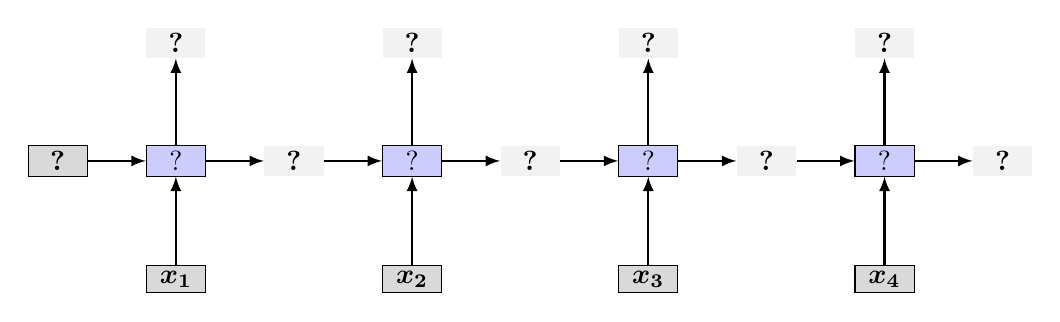
\begin{tikzpicture}	
	%\node (a1) [draw, circle, inner sep=0pt, minimum width=0.75cm, fill=green!20] {$a_1$};
	
	\node (s0) [constant]{$\bm{?}$};
	
	\node (ro1) [neuron, right of=s0, xshift=0.5cm] {$?$};
	\node (s1) [state, right of=ro1, xshift=0.5cm] {$\bm{?}$};
	\node (x1) [constant, below of=ro1, yshift=-0.5cm] {$\bm{x_1}$};
	\node(y1) [state, above of=ro1, yshift=0.5cm] {$\bm{?}$};
	
	\node (ro2) [neuron, right of=s1, xshift=0.5cm] {$?$};
	\node (s2) [state, right of=ro2, xshift=0.5cm] {$\bm{?}$};
	\node (x2) [constant, below of=ro2, yshift=-0.5cm] {$\bm{x_2}$};
	\node(y2) [state, above of=ro2, yshift=0.5cm] {$\bm{?}$};
	
	\node (ro3) [neuron, right of=s2, xshift=0.5cm] {$?$};
	\node (s3) [state, right of=ro3, xshift=0.5cm] {$\bm{?}$};
	\node (x3) [constant, below of=ro3, yshift=-0.5cm] {$\bm{x_3}$};
	\node(y3) [state, above of=ro3, yshift=0.5cm] {$\bm{?}$};
	
	\node (ro4) [neuron, right of=s3, xshift=0.5cm] {$?$};
	\node (s4) [state, right of=ro4, xshift=0.5cm] {$\bm{?}$};
	\node (x4) [constant, below of=ro4, yshift=-0.5cm] {$\bm{x_4}$};
	\node(y4) [state, above of=ro4, yshift=0.5cm] {$\bm{?}$};
		
	
	\begin{scope}[thick, black, ->, >=latex]
		\draw (s0) -- (ro1);
		\draw(x1) -- (ro1);
		\draw(ro1) -- (s1);
		\draw(ro1) -- (y1);
		
		\draw (s1) -- (ro2);
		\draw(x2) -- (ro2);
		\draw(ro2) -- (s2);
		\draw(ro2) -- (y2);
		
		\draw (s2) -- (ro3);
		\draw(x3) -- (ro3);
		\draw(ro3) -- (s3);
		\draw(ro3) -- (y3);
		
		\draw (s3) -- (ro4);
		\draw(x4) -- (ro4);
		\draw(ro4) -- (s4);
		\draw(ro4) -- (y4);
		
	\end{scope}
	
\end{tikzpicture}
Example for 4 input tokens


\end{frame}


\begin{frame}{RNN abstraction}

We have a sequence of $n$ \textbf{input} vectors $\bm{x_{1:n}} = \bm{x_1}, \ldots, \bm{x_n}$

Each input vector has the same dimension $d_{in}: \bm{x_i} \in \mathbb{R}^{d_{in}}$

\bigskip

What might $\bm{x_i}$ contain?
\begin{itemize}
	\item Typically a word embedding of token $i$, but could be any arbitrary input, e.g., one-hot encoding of token $i$
\end{itemize}
\bigskip

\pause

Output: a vector $\bm{y_i} \in \mathbb{R}^{d_{out}}$ at each position $i \in (1, \ldots, n)$

Let's call this sequence-outputting function $\rnnstar$:
$$
\bm{y_{1:n}} = \rnnstar (\bm{x_{1:n}})
$$

\end{frame}



\begin{frame}{Adding outputs to our sketch}

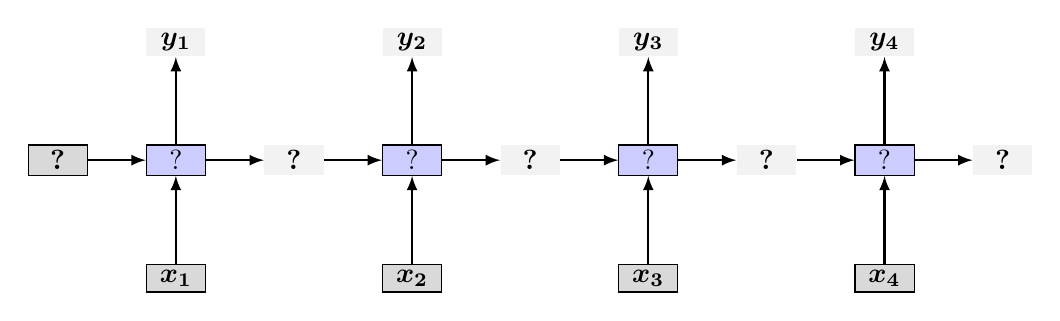
\begin{tikzpicture}	
	%\node (a1) [draw, circle, inner sep=0pt, minimum width=0.75cm, fill=green!20] {$a_1$};
	
	\node (s0) [constant]{$\bm{?}$};
	
	\node (ro1) [neuron, right of=s0, xshift=0.5cm] {$?$};
	\node (s1) [state, right of=ro1, xshift=0.5cm] {$\bm{?}$};
	\node (x1) [constant, below of=ro1, yshift=-0.5cm] {$\bm{x_1}$};
	\node(y1) [state, above of=ro1, yshift=0.5cm] {$\bm{y_1}$};
	
	\node (ro2) [neuron, right of=s1, xshift=0.5cm] {$?$};
	\node (s2) [state, right of=ro2, xshift=0.5cm] {$\bm{?}$};
	\node (x2) [constant, below of=ro2, yshift=-0.5cm] {$\bm{x_2}$};
	\node(y2) [state, above of=ro2, yshift=0.5cm] {$\bm{y_2}$};
	
	\node (ro3) [neuron, right of=s2, xshift=0.5cm] {$?$};
	\node (s3) [state, right of=ro3, xshift=0.5cm] {$\bm{?}$};
	\node (x3) [constant, below of=ro3, yshift=-0.5cm] {$\bm{x_3}$};
	\node(y3) [state, above of=ro3, yshift=0.5cm] {$\bm{y_3}$};
	
	\node (ro4) [neuron, right of=s3, xshift=0.5cm] {$?$};
	\node (s4) [state, right of=ro4, xshift=0.5cm] {$\bm{?}$};
	\node (x4) [constant, below of=ro4, yshift=-0.5cm] {$\bm{x_4}$};
	\node(y4) [state, above of=ro4, yshift=0.5cm] {$\bm{y_4}$};
	
	
	\begin{scope}[thick, black, ->, >=latex]
		\draw (s0) -- (ro1);
		\draw(x1) -- (ro1);
		\draw(ro1) -- (s1);
		\draw(ro1) -- (y1);
		
		\draw (s1) -- (ro2);
		\draw(x2) -- (ro2);
		\draw(ro2) -- (s2);
		\draw(ro2) -- (y2);
		
		\draw (s2) -- (ro3);
		\draw(x3) -- (ro3);
		\draw(ro3) -- (s3);
		\draw(ro3) -- (y3);
		
		\draw (s3) -- (ro4);
		\draw(x4) -- (ro4);
		\draw(ro4) -- (s4);
		\draw(ro4) -- (y4);
		
	\end{scope}
	
\end{tikzpicture}



\end{frame}


\begin{frame}{Recap}

For a sequence of input vectors  $\bm{x_{1:i}}$
$$
\bm{y_{1:n}} = \rnnstar (\bm{x_{1:n}})
$$

\pause

Without knowing what $\rnn$ actually is, what are the advantages?
\pause
\begin{itemize}
	\item Each output $\bm{y_i}$ takes into account the entire history $\bm{x_{1:i}}$ without Markov property
\end{itemize}

What to do with $\bm{y_n}$ or $\bm{y_{1:n}}$?
\pause
\begin{itemize}
	\item Use for further prediction, e.g., plug into $\softmax$, MLP, etc.
\end{itemize}

\end{frame}



\begin{frame}{Underlying mechanism of RNNs --- states}
For ``passing information'' from one position to the next, i.e.\ from
$$\bm{y_i} = \rnn (\bm{x_{1:i}})$$
to
$$\bm{y_{i+1}} = \rnn (\bm{x_{1:i+1}})$$
we use a ``state'' vector
$$\bm{s_i} \in \mathbb{R}^{d_{state}}$$
\end{frame}


\begin{frame}{Adding state vectors}

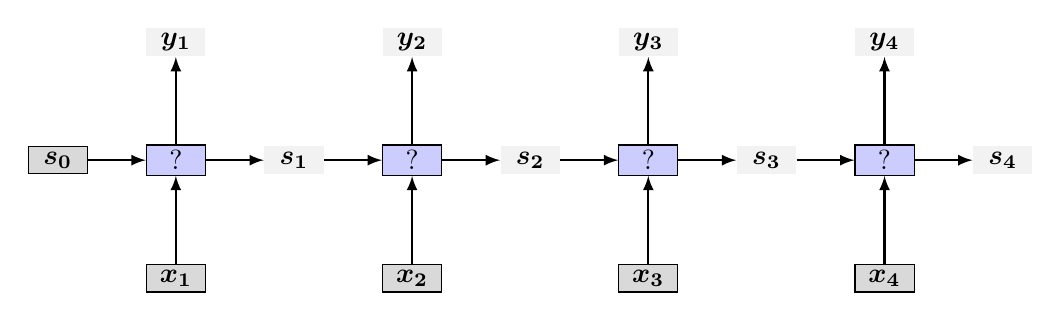
\begin{tikzpicture}	
	%\node (a1) [draw, circle, inner sep=0pt, minimum width=0.75cm, fill=green!20] {$a_1$};
	
	\node (s0) [constant]{$\bm{s_0}$};
	
	\node (ro1) [neuron, right of=s0, xshift=0.5cm] {$?$};
	\node (s1) [state, right of=ro1, xshift=0.5cm] {$\bm{s_1}$};
	\node (x1) [constant, below of=ro1, yshift=-0.5cm] {$\bm{x_1}$};
	\node(y1) [state, above of=ro1, yshift=0.5cm] {$\bm{y_1}$};
	
	\node (ro2) [neuron, right of=s1, xshift=0.5cm] {$?$};
	\node (s2) [state, right of=ro2, xshift=0.5cm] {$\bm{s_2}$};
	\node (x2) [constant, below of=ro2, yshift=-0.5cm] {$\bm{x_2}$};
	\node(y2) [state, above of=ro2, yshift=0.5cm] {$\bm{y_2}$};
	
	\node (ro3) [neuron, right of=s2, xshift=0.5cm] {$?$};
	\node (s3) [state, right of=ro3, xshift=0.5cm] {$\bm{s_3}$};
	\node (x3) [constant, below of=ro3, yshift=-0.5cm] {$\bm{x_3}$};
	\node(y3) [state, above of=ro3, yshift=0.5cm] {$\bm{y_3}$};
	
	\node (ro4) [neuron, right of=s3, xshift=0.5cm] {$?$};
	\node (s4) [state, right of=ro4, xshift=0.5cm] {$\bm{s_4}$};
	\node (x4) [constant, below of=ro4, yshift=-0.5cm] {$\bm{x_4}$};
	\node(y4) [state, above of=ro4, yshift=0.5cm] {$\bm{y_4}$};
	
	
	
	\begin{scope}[thick, black, ->, >=latex]
		\draw (s0) -- (ro1);
		\draw(x1) -- (ro1);
		\draw(ro1) -- (s1);
		\draw(ro1) -- (y1);
		
		\draw (s1) -- (ro2);
		\draw(x2) -- (ro2);
		\draw(ro2) -- (s2);
		\draw(ro2) -- (y2);
		
		\draw (s2) -- (ro3);
		\draw(x3) -- (ro3);
		\draw(ro3) -- (s3);
		\draw(ro3) -- (y3);
		
		\draw (s3) -- (ro4);
		\draw(x4) -- (ro4);
		\draw(ro4) -- (s4);
		\draw(ro4) -- (y4);
		
	\end{scope}
	
\end{tikzpicture}



\end{frame}



\begin{frame}{Define RNN recursively --- Computing current state}
At each step $i \in (1, \ldots, n)$ we have
\begin{itemize}
	\item Current input vector $\bm{x_i}$
	\item Vector of the previous state $\bm{s_{i - 1}}$\footnote{Initial state vector $\bm{s_0}$ --- often omitted, assumed to be zero-filled}
\end{itemize}
and compute
\begin{itemize}
	\item Current state $\bm{s_i}$
\end{itemize}
$$
\bm{s_i} = R(\bm{s_{i-1}}, \bm{x_i}) \qquad \text{(we will specify $R$ later)}
$$

\end{frame}


\begin{frame}{Define RNN recursively --- Computing current output}
At each step $i \in (1, \ldots, n)$ we have
\begin{itemize}
	\item Current input vector $\bm{x_i}$
	\item Vector of the previous state $\bm{s_{i - 1}}$
\end{itemize}
and compute
\begin{itemize}
	\item Current state $\bm{s_i} = R(\bm{s_{i-1}}, \bm{x_i})$
	\item Current output $\bm{y_i}$
\end{itemize}
$$
\bm{y_i} = O(\bm{s_i}) \qquad \text{(we will specify $O$ later)}
$$

\end{frame}



\begin{frame}{Adding $R$ and $O$}

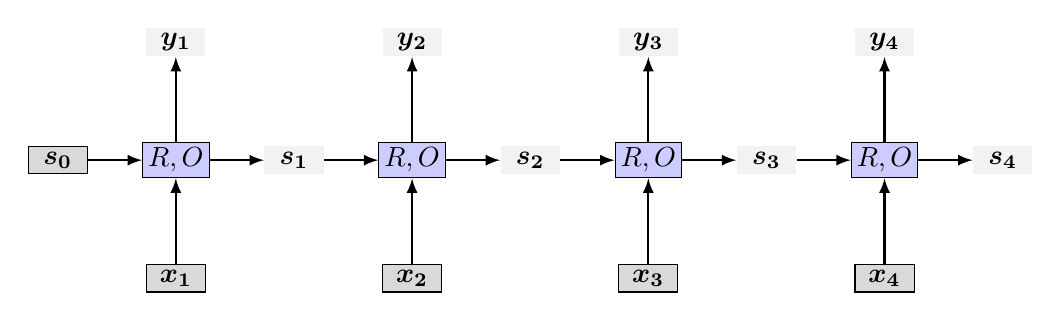
\begin{tikzpicture}	
	%\node (a1) [draw, circle, inner sep=0pt, minimum width=0.75cm, fill=green!20] {$a_1$};
	
	\node (s0) [constant]{$\bm{s_0}$};
	
	\node (ro1) [neuron, right of=s0, xshift=0.5cm] {$R, O$};
	\node (s1) [state, right of=ro1, xshift=0.5cm] {$\bm{s_1}$};
	\node (x1) [constant, below of=ro1, yshift=-0.5cm] {$\bm{x_1}$};
	\node(y1) [state, above of=ro1, yshift=0.5cm] {$\bm{y_1}$};
	
	\node (ro2) [neuron, right of=s1, xshift=0.5cm] {$R, O$};
	\node (s2) [state, right of=ro2, xshift=0.5cm] {$\bm{s_2}$};
	\node (x2) [constant, below of=ro2, yshift=-0.5cm] {$\bm{x_2}$};
	\node(y2) [state, above of=ro2, yshift=0.5cm] {$\bm{y_2}$};
	
	\node (ro3) [neuron, right of=s2, xshift=0.5cm] {$R, O$};
	\node (s3) [state, right of=ro3, xshift=0.5cm] {$\bm{s_3}$};
	\node (x3) [constant, below of=ro3, yshift=-0.5cm] {$\bm{x_3}$};
	\node(y3) [state, above of=ro3, yshift=0.5cm] {$\bm{y_3}$};
	
	\node (ro4) [neuron, right of=s3, xshift=0.5cm] {$R, O$};
	\node (s4) [state, right of=ro4, xshift=0.5cm] {$\bm{s_4}$};
	\node (x4) [constant, below of=ro4, yshift=-0.5cm] {$\bm{x_4}$};
	\node(y4) [state, above of=ro4, yshift=0.5cm] {$\bm{y_4}$};
	
	
	\begin{scope}[thick, black, ->, >=latex]
		\draw (s0) -- (ro1);
		\draw(x1) -- (ro1);
		\draw(ro1) -- (s1);
		\draw(ro1) -- (y1);
		
		\draw (s1) -- (ro2);
		\draw(x2) -- (ro2);
		\draw(ro2) -- (s2);
		\draw(ro2) -- (y2);
		
		\draw (s2) -- (ro3);
		\draw(x3) -- (ro3);
		\draw(ro3) -- (s3);
		\draw(ro3) -- (y3);
		
		\draw (s3) -- (ro4);
		\draw(x4) -- (ro4);
		\draw(ro4) -- (s4);
		\draw(ro4) -- (y4);
		
	\end{scope}
	
\end{tikzpicture}



\end{frame}


\begin{frame}{Summary}
At each step $i \in (1, \ldots, n)$ we have
\begin{itemize}
	\item Current input $\bm{x_i}$ and previous state $\bm{s_{i - 1}}$
\end{itemize}
and compute
\begin{itemize}
	\item $\bm{s_i} = R(\bm{s_{i-1}}, \bm{x_i})$ and $\bm{y_i}  = O(\bm{s_i})$
\end{itemize}

The functions $R$ and $O$ are the same for each position $i$

\begin{block}{RNN}
	$\bm{y_{1:n}} = \rnnstar (\bm{x_{1:n}}, \bm{s_0})
	\qquad
	\bm{s_i} = R(\bm{s_{i-1}}, \bm{x_i})
	\qquad
	\bm{y_i}  = O(\bm{s_i})$
\end{block}


\end{frame}


\begin{frame}{Graphical visualization of abstract RNN (unrolled)}

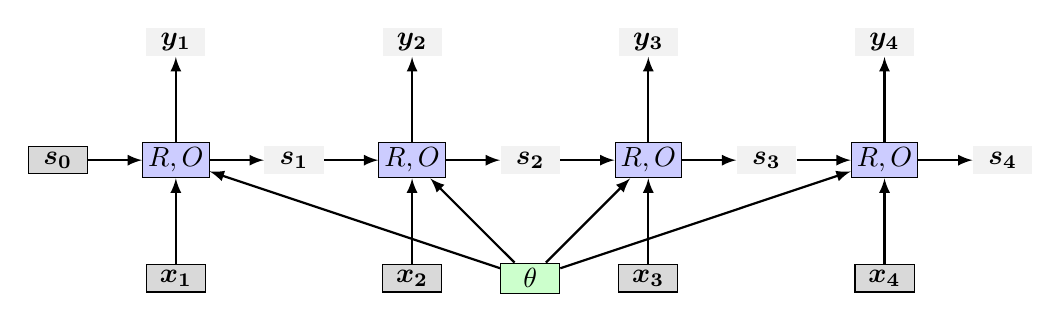
\begin{tikzpicture}	
	%\node (a1) [draw, circle, inner sep=0pt, minimum width=0.75cm, fill=green!20] {$a_1$};
	
	\node (s0) [constant]{$\bm{s_0}$};
	
	\node (ro1) [neuron, right of=s0, xshift=0.5cm] {$R, O$};
	\node (s1) [state, right of=ro1, xshift=0.5cm] {$\bm{s_1}$};
	\node (x1) [constant, below of=ro1, yshift=-0.5cm] {$\bm{x_1}$};
	\node(y1) [state, above of=ro1, yshift=0.5cm] {$\bm{y_1}$};
	
	\node (ro2) [neuron, right of=s1, xshift=0.5cm] {$R, O$};
	\node (s2) [state, right of=ro2, xshift=0.5cm] {$\bm{s_2}$};
	\node (x2) [constant, below of=ro2, yshift=-0.5cm] {$\bm{x_2}$};
	\node(y2) [state, above of=ro2, yshift=0.5cm] {$\bm{y_2}$};
	
	\node (ro3) [neuron, right of=s2, xshift=0.5cm] {$R, O$};
	\node (s3) [state, right of=ro3, xshift=0.5cm] {$\bm{s_3}$};
	\node (x3) [constant, below of=ro3, yshift=-0.5cm] {$\bm{x_3}$};
	\node(y3) [state, above of=ro3, yshift=0.5cm] {$\bm{y_3}$};
	
	\node (ro4) [neuron, right of=s3, xshift=0.5cm] {$R, O$};
	\node (s4) [state, right of=ro4, xshift=0.5cm] {$\bm{s_4}$};
	\node (x4) [constant, below of=ro4, yshift=-0.5cm] {$\bm{x_4}$};
	\node(y4) [state, above of=ro4, yshift=0.5cm] {$\bm{y_4}$};
	
	\node (e) [param, below of=s2, yshift=-0.5cm] {$\theta$};
	
	
	\begin{scope}[thick, black, ->, >=latex]
		\draw (s0) -- (ro1);
		\draw(x1) -- (ro1);
		\draw(e) -- (ro1);
		\draw(ro1) -- (s1);
		\draw(ro1) -- (y1);
		
		\draw (s1) -- (ro2);
		\draw(x2) -- (ro2);
		\draw(e) -- (ro2);
		\draw(ro2) -- (s2);
		\draw(ro2) -- (y2);
		
		\draw (s2) -- (ro3);
		\draw(x3) -- (ro3);
		\draw(e) -- (ro3);
		\draw(ro3) -- (s3);
		\draw(ro3) -- (y3);
		
		\draw (s3) -- (ro4);
		\draw(x4) -- (ro4);
		\draw(e) -- (ro4);
		\draw(ro4) -- (s4);
		\draw(ro4) -- (y4);
		
	\end{scope}
	
\end{tikzpicture}

\bigskip
\pause
Note that $\theta$ (parameters) are ``shared" (the same) for all positions


\end{frame}


\begin{frame}{Graphical visualization of abstract RNN (recursive)}

\begin{figure}
	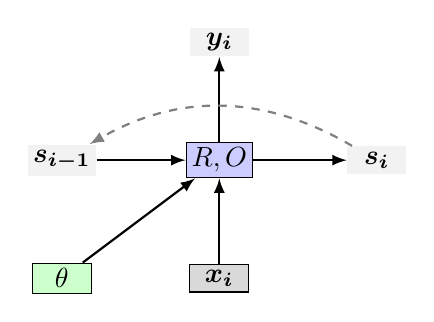
\begin{tikzpicture}	
		%\node (a1) [draw, circle, inner sep=0pt, minimum width=0.75cm, fill=green!20] {$a_1$};
		
		\node (s0) [state]{$\bm{s_{i-1}}$};
		\node (e) [param, below of=s0, yshift=-0.5cm] {$\theta$};
		
		\node (ro) [neuron, right of=s0, xshift=1cm] {$R, O$};
		\node (si) [state, right of=ro, xshift=1cm] {$\bm{s_{i}}$};
		\node (xi) [constant, below of=ro, yshift=-0.5cm] {$\bm{x_{i}}$};
		\node(yi) [state, above of=ro, yshift=0.5cm] {$\bm{y_i}$};
		
		\begin{scope}[thick, black, ->, >=latex]
			\draw (s0) -- (ro);
			\draw(xi) -- (ro);
			\draw(e) -- (ro);
			\draw(ro) -- (si);
			\draw(ro) -- (yi);
		\end{scope}
		\draw [thick, dashed, gray, ->, >=latex] (si) to [bend right] (s0);
		
	\end{tikzpicture}
\end{figure}

\end{frame}




\subsection{RNN as `acceptor' or `encoder'}


\begin{frame}{Supervision on the last output}


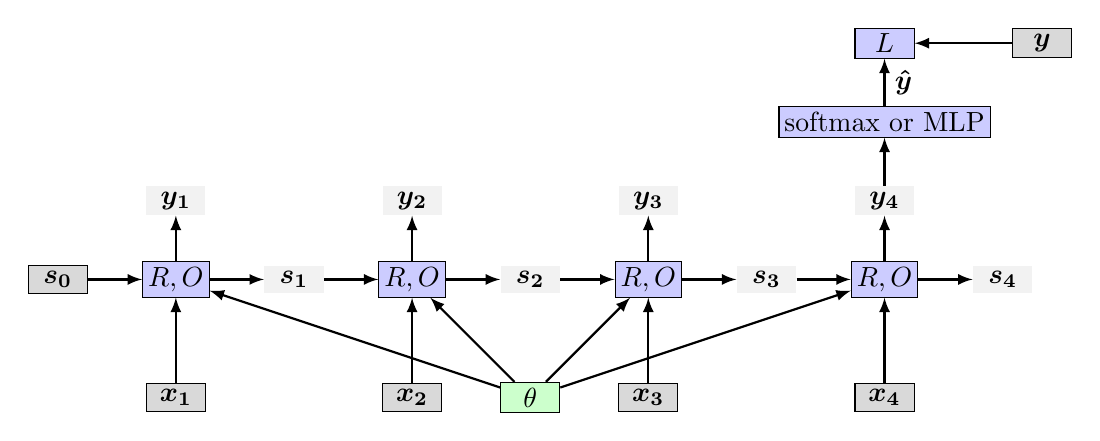
\begin{tikzpicture}	
	%\node (a1) [draw, circle, inner sep=0pt, minimum width=0.75cm, fill=green!20] {$a_1$};
	
	\node (s0) [constant]{$\bm{s_0}$};
	
	\node (ro1) [neuron, right of=s0, xshift=0.5cm] {$R, O$};
	\node (s1) [state, right of=ro1, xshift=0.5cm] {$\bm{s_1}$};
	\node (x1) [constant, below of=ro1, yshift=-0.5cm] {$\bm{x_1}$};
	\node(y1) [state, above of=ro1, yshift=0cm] {$\bm{y_1}$};
	
	\node (ro2) [neuron, right of=s1, xshift=0.5cm] {$R, O$};
	\node (s2) [state, right of=ro2, xshift=0.5cm] {$\bm{s_2}$};
	\node (x2) [constant, below of=ro2, yshift=-0.5cm] {$\bm{x_2}$};
	\node(y2) [state, above of=ro2, yshift=0cm] {$\bm{y_2}$};
	
	\node (ro3) [neuron, right of=s2, xshift=0.5cm] {$R, O$};
	\node (s3) [state, right of=ro3, xshift=0.5cm] {$\bm{s_3}$};
	\node (x3) [constant, below of=ro3, yshift=-0.5cm] {$\bm{x_3}$};
	\node(y3) [state, above of=ro3, yshift=0cm] {$\bm{y_3}$};
	
	\node (ro4) [neuron, right of=s3, xshift=0.5cm] {$R, O$};
	\node (s4) [state, right of=ro4, xshift=0.5cm] {$\bm{s_4}$};
	\node (x4) [constant, below of=ro4, yshift=-0.5cm] {$\bm{x_4}$};
	\node(y4) [state, above of=ro4, yshift=0cm] {$\bm{y_4}$};
	
	\node (e) [param, below of=s2, yshift=-0.5cm] {$\theta$};
	
	
	\node (mlp) [neuron, above of=y4] {$\softmax$ or MLP};
	
	\node (l) [neuron, above of=mlp] {$L$};
	\node (y) [constant, right of=l, xshift=1cm] {$\bm{y}$};
	
	
	\begin{scope}[thick, black, ->, >=latex]
		\draw (s0) -- (ro1);
		\draw(x1) -- (ro1);
		\draw(e) -- (ro1);
		\draw(ro1) -- (s1);
		\draw(ro1) -- (y1);
		
		\draw (s1) -- (ro2);
		\draw(x2) -- (ro2);
		\draw(e) -- (ro2);
		\draw(ro2) -- (s2);
		\draw(ro2) -- (y2);
		
		\draw (s2) -- (ro3);
		\draw(x3) -- (ro3);
		\draw(e) -- (ro3);
		\draw(ro3) -- (s3);
		\draw(ro3) -- (y3);
		
		\draw (s3) -- (ro4);
		\draw(x4) -- (ro4);
		\draw(e) -- (ro4);
		\draw(ro4) -- (s4);
		\draw(ro4) -- (y4);
		
		\draw (y4) -- (mlp);
		\draw (mlp) -- (l) node [midway, right] {$\bm{\hat{y}}$};
		\draw (y) -- (l);
		
	\end{scope}
	
	
	
\end{tikzpicture}



The loss is computed on the final output (e.g., directly on $\bm{y_n}$ or by putting $\bm{y_n}$ through MLP)



\end{frame}


\subsection{RNN as `transducer'}


\begin{frame}{Supervision on each output}


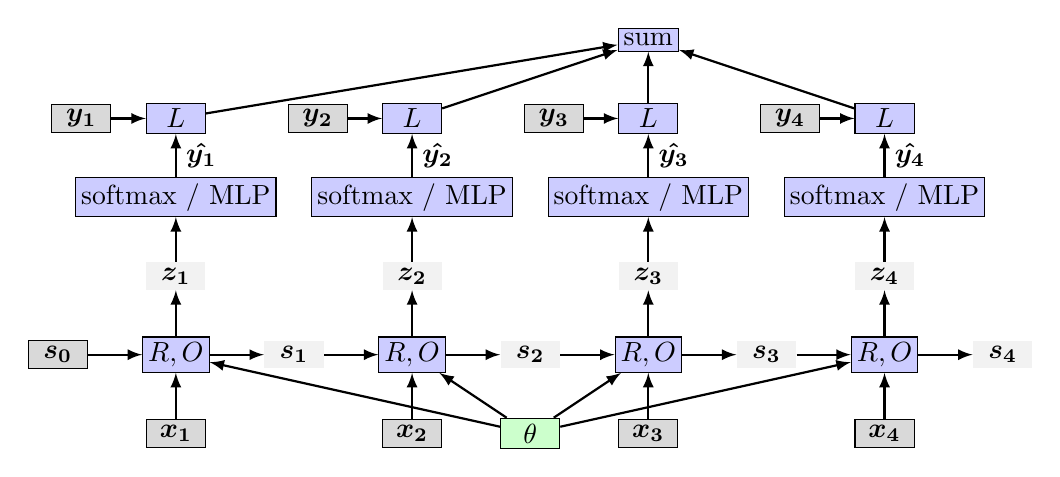
\begin{tikzpicture}	
	%\node (a1) [draw, circle, inner sep=0pt, minimum width=0.75cm, fill=green!20] {$a_1$};
	
	\node (s0) [constant]{$\bm{s_0}$};
	
	\node (ro1) [neuron, right of=s0, xshift=0.5cm] {$R, O$};
	\node (s1) [state, right of=ro1, xshift=0.5cm] {$\bm{s_1}$};
	\node (x1) [constant, below of=ro1, yshift=-0cm] {$\bm{x_1}$};
	\node(y1) [state, above of=ro1, yshift=0cm] {$\bm{z_1}$};
	
	\node (ro2) [neuron, right of=s1, xshift=0.5cm] {$R, O$};
	\node (s2) [state, right of=ro2, xshift=0.5cm] {$\bm{s_2}$};
	\node (x2) [constant, below of=ro2, yshift=-0cm] {$\bm{x_2}$};
	\node(y2) [state, above of=ro2, yshift=0cm] {$\bm{z_2}$};
	
	\node (ro3) [neuron, right of=s2, xshift=0.5cm] {$R, O$};
	\node (s3) [state, right of=ro3, xshift=0.5cm] {$\bm{s_3}$};
	\node (x3) [constant, below of=ro3, yshift=-0cm] {$\bm{x_3}$};
	\node(y3) [state, above of=ro3, yshift=0cm] {$\bm{z_3}$};
	
	\node (ro4) [neuron, right of=s3, xshift=0.5cm] {$R, O$};
	\node (s4) [state, right of=ro4, xshift=0.5cm] {$\bm{s_4}$};
	\node (x4) [constant, below of=ro4, yshift=-0cm] {$\bm{x_4}$};
	\node(y4) [state, above of=ro4, yshift=0cm] {$\bm{z_4}$};
	
	\node (e) [param, below of=s2, yshift=-0cm] {$\theta$};
	
	
	\node (mlp1) [neuron, above of=y1] {$\softmax$ / MLP};
	\node (mlp2) [neuron, above of=y2] {$\softmax$ / MLP};
	\node (mlp3) [neuron, above of=y3] {$\softmax$ / MLP};
	\node (mlp4) [neuron, above of=y4] {$\softmax$ / MLP};
	
	\node (l1) [neuron, above of=mlp1] {$L$};
	\node (l2) [neuron, above of=mlp2] {$L$};
	\node (l3) [neuron, above of=mlp3] {$L$};
	\node (l4) [neuron, above of=mlp4] {$L$};
	
	\node (yg1) [constant, left of=l1, xshift=-0.2cm] {$\bm{y_1}$};
	\node (yg2) [constant, left of=l2, xshift=-0.2cm] {$\bm{y_2}$};
	\node (yg3) [constant, left of=l3, xshift=-0.2cm] {$\bm{y_3}$};
	\node (yg4) [constant, left of=l4, xshift=-0.2cm] {$\bm{y_4}$};
	
	\node (sum) [neuron, above of=l3] {sum};
	
	\begin{scope}[thick, black, ->, >=latex]
		\draw (s0) -- (ro1);
		\draw(x1) -- (ro1);
		\draw(e) -- (ro1);
		\draw(ro1) -- (s1);
		\draw(ro1) -- (y1);
		
		\draw (s1) -- (ro2);
		\draw(x2) -- (ro2);
		\draw(e) -- (ro2);
		\draw(ro2) -- (s2);
		\draw(ro2) -- (y2);
		
		\draw (s2) -- (ro3);
		\draw(x3) -- (ro3);
		\draw(e) -- (ro3);
		\draw(ro3) -- (s3);
		\draw(ro3) -- (y3);
		
		\draw (s3) -- (ro4);
		\draw(x4) -- (ro4);
		\draw(e) -- (ro4);
		\draw(ro4) -- (s4);
		\draw(ro4) -- (y4);
		
		\draw (y1) -- (mlp1);
		\draw (y2) -- (mlp2);
		\draw (y3) -- (mlp3);
		\draw (y4) -- (mlp4);
		
		\draw (mlp1) -- (l1) node [midway, right] {$\bm{\hat{y_1}}$};
		\draw (mlp2) -- (l2) node [midway, right] {$\bm{\hat{y_2}}$};
		\draw (mlp3) -- (l3) node [midway, right] {$\bm{\hat{y_3}}$};
		\draw (mlp4) -- (l4) node [midway, right] {$\bm{\hat{y_4}}$};
		
		\draw (yg1) -- (l1);
		\draw (yg2) -- (l2);
		\draw (yg3) -- (l3);
		\draw (yg4) -- (l4);
		
		\draw (l1) -- (sum);
		\draw (l2) -- (sum);
		\draw (l3) -- (sum);
		\draw (l4) -- (sum);
		
	\end{scope}
	
	
	
\end{tikzpicture}

For sequence tagging --- loss on each position, overall network's loss simply as a sum of losses


\end{frame}

\begin{frame}{Bi-directional RNNs}
Simple idea: Run one RNN from left-to-right (forward, $f$) and another RNN from right-to-left (backward, $b$), and concatenate
$$
\birnn (\bm{x_{1:i}}, i) = \bm{y_i} = [
\rnn_f(\bm{x_{1:i}});
\rnn_b(\bm{x_{n:i}})
]
$$

Both for encoder (concatenate the last outputs) and transducer (concatenate each step's output)

\end{frame}

\begin{frame}{But what is happening `inside' $R$ and $O$?}
\begin{figure}
	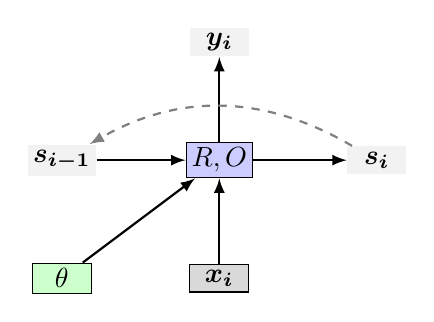
\begin{tikzpicture}	
		%\node (a1) [draw, circle, inner sep=0pt, minimum width=0.75cm, fill=green!20] {$a_1$};
		
		\node (s0) [state]{$\bm{s_{i-1}}$};
		\node (e) [param, below of=s0, yshift=-0.5cm] {$\theta$};
		
		\node (ro) [neuron, right of=s0, xshift=1cm] {$R, O$};
		\node (si) [state, right of=ro, xshift=1cm] {$\bm{s_{i}}$};
		\node (xi) [constant, below of=ro, yshift=-0.5cm] {$\bm{x_{i}}$};
		\node(yi) [state, above of=ro, yshift=0.5cm] {$\bm{y_i}$};
		
		\begin{scope}[thick, black, ->, >=latex]
			\draw (s0) -- (ro);
			\draw(xi) -- (ro);
			\draw(e) -- (ro);
			\draw(ro) -- (si);
			\draw(ro) -- (yi);
		\end{scope}
		\draw [thick, dashed, gray, ->, >=latex] (si) to [bend right] (s0);
		
	\end{tikzpicture}
\end{figure}
\end{frame}

\section{RNN architectures}


\subsection{Simple RNN}

\begin{frame}{Elman Network or Simple-RNN (S-RNN)}
\begin{figure}
	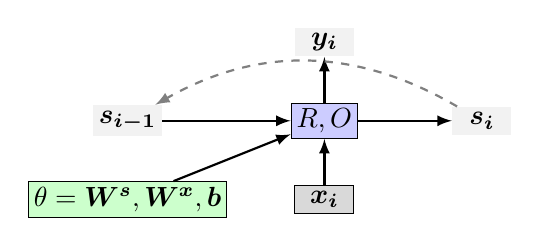
\begin{tikzpicture}	
		%\node (a1) [draw, circle, inner sep=0pt, minimum width=0.75cm, fill=green!20] {$a_1$};
		
		\node (s0) [state]{$\bm{s_{i-1}}$};
		\node (e) [param, below of=s0] {$\theta = \bm{W^s}, \bm{W^x}, \bm{b}$};
		
		\node (ro) [neuron, right of=s0, xshift=1.5cm] {$R, O$};
		\node (si) [state, right of=ro, xshift=1cm] {$\bm{s_{i}}$};
		\node (xi) [constant, below of=ro] {$\bm{x_{i}}$};
		\node(yi) [state, above of=ro] {$\bm{y_i}$};
		
		\begin{scope}[thick, black, ->, >=latex]
			\draw (s0) -- (ro);
			\draw(xi) -- (ro);
			\draw(e) -- (ro);
			\draw(ro) -- (si);
			\draw(ro) -- (yi);
		\end{scope}
		\draw [thick, dashed, gray, ->, >=latex] (si) to [bend right] (s0);
		
	\end{tikzpicture}
\end{figure}
$$
\begin{aligned}
	\bm{s_i} &= R(\bm{x_i}, \bm{s_{i - 1}}) = g(\bm{s_{i-1}} \bm{W^s} + \bm{x_i} \bm{W^x} + \bm{b}) \\
	\bm{y_i} &= O(\bm{s_i}) = \bm{s_i}
\end{aligned}
$$
\bigskip
\pause
$$
\bm{s_i}, \bm{y_i} \in \mathbb{R}^d_s \quad
\bm{x_i} \in \mathbb{R}^d_{in} \quad
\bm{W^x} \in \mathbb{R}^{d_{in} \times d_s} \quad
\bm{W^s} \in \mathbb{R}^{d_s \times d_s} \quad
\bm{b} \in \mathbb{R}^{d_s}
$$
$g$ --- commonly tanh or ReLU


\end{frame}


\begin{frame}{Elman Network and vanishing gradient}
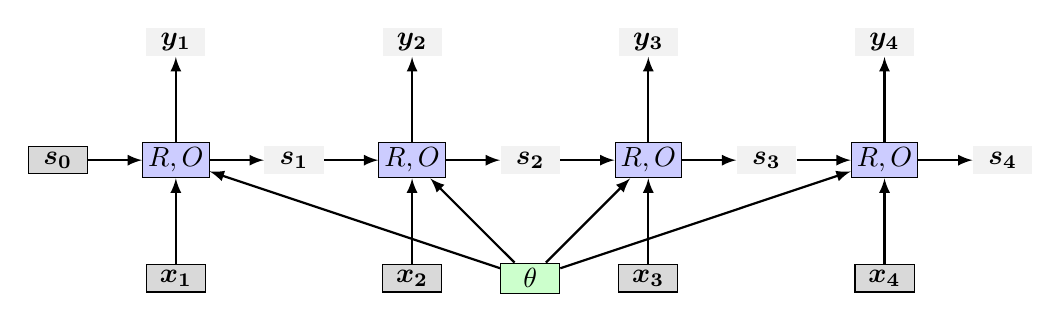
\begin{tikzpicture}	
	%\node (a1) [draw, circle, inner sep=0pt, minimum width=0.75cm, fill=green!20] {$a_1$};
	
	\node (s0) [constant]{$\bm{s_0}$};
	
	\node (ro1) [neuron, right of=s0, xshift=0.5cm] {$R, O$};
	\node (s1) [state, right of=ro1, xshift=0.5cm] {$\bm{s_1}$};
	\node (x1) [constant, below of=ro1, yshift=-0.5cm] {$\bm{x_1}$};
	\node(y1) [state, above of=ro1, yshift=0.5cm] {$\bm{y_1}$};
	
	\node (ro2) [neuron, right of=s1, xshift=0.5cm] {$R, O$};
	\node (s2) [state, right of=ro2, xshift=0.5cm] {$\bm{s_2}$};
	\node (x2) [constant, below of=ro2, yshift=-0.5cm] {$\bm{x_2}$};
	\node(y2) [state, above of=ro2, yshift=0.5cm] {$\bm{y_2}$};
	
	\node (ro3) [neuron, right of=s2, xshift=0.5cm] {$R, O$};
	\node (s3) [state, right of=ro3, xshift=0.5cm] {$\bm{s_3}$};
	\node (x3) [constant, below of=ro3, yshift=-0.5cm] {$\bm{x_3}$};
	\node(y3) [state, above of=ro3, yshift=0.5cm] {$\bm{y_3}$};
	
	\node (ro4) [neuron, right of=s3, xshift=0.5cm] {$R, O$};
	\node (s4) [state, right of=ro4, xshift=0.5cm] {$\bm{s_4}$};
	\node (x4) [constant, below of=ro4, yshift=-0.5cm] {$\bm{x_4}$};
	\node(y4) [state, above of=ro4, yshift=0.5cm] {$\bm{y_4}$};
	
	\node (e) [param, below of=s2, yshift=-0.5cm] {$\theta$};
	
	
	\begin{scope}[thick, black, ->, >=latex]
		\draw (s0) -- (ro1);
		\draw(x1) -- (ro1);
		\draw(e) -- (ro1);
		\draw(ro1) -- (s1);
		\draw(ro1) -- (y1);
		
		\draw (s1) -- (ro2);
		\draw(x2) -- (ro2);
		\draw(e) -- (ro2);
		\draw(ro2) -- (s2);
		\draw(ro2) -- (y2);
		
		\draw (s2) -- (ro3);
		\draw(x3) -- (ro3);
		\draw(e) -- (ro3);
		\draw(ro3) -- (s3);
		\draw(ro3) -- (y3);
		
		\draw (s3) -- (ro4);
		\draw(x4) -- (ro4);
		\draw(e) -- (ro4);
		\draw(ro4) -- (s4);
		\draw(ro4) -- (y4);
		
	\end{scope}
	
\end{tikzpicture}

Gradients might vanish ($\to 0$) as they propagate back through the computation graph

\begin{itemize}
	\item Severe in deeper nets, especially in recurrent networks
	\item Hard for the S-RNN to capture long-range dependencies
\end{itemize}



\end{frame}

\subsection{Gated architectures}

\begin{frame}{RNN as a general purpose computing device}

State $\bm{s_i}$ represents a finite memory

\begin{block}{Recall: Simple RNN}
	$\bm{s_i} = R(\bm{x_i}, \bm{s_{i - 1}}) = g(\bm{s_{i-1}} \bm{W^s} + \bm{x_i} \bm{W^x} + \bm{b})$ 	
\end{block}
\pause
Each application of function $R$
\begin{itemize}
	\item Reads the current memory $\bm{s_{i-1}}$
	\item Reads the current input $\bm{x_i}$
	\item Operates on them in some way
	\item Writes the result to the memory $\bm{s_i}$
\end{itemize}
\pause Memory access not controlled: At each step, entire memory state is read, and entire memory state is written
\end{frame}

\begin{frame}{How to provide more controlled memory access?}
Memory vector $\bm{s} \in \mathbb{R}^d$ and input vector $\bm{x} \in \mathbb{R}^d$
\pause

Let's have a binary vector (``gate'') $\bm{g} \in \{0, 1\}^d$
\pause
\begin{block}{Hadamard-product $\bm{z} = \bm{u} \odot \bm{v}$}
	Fancy name for element-wise multiplication
	$\bm{z_{[i]}} = \bm{u_{[i]}} \cdot \bm{v_{[i]}}$
\end{block}
$
\bm{s'} \gets \bm{g} \odot \bm{x} + (\bm{1} + \bm{g}) \odot \bm{s}
$
\begin{itemize}
	\item \pause Reads the entries in $\bm{x}$ corresponding to ones in the gate, writes them to the memory
	\item \pause Remaining locations are copied from the memory
\item Note that the operation $+$ here is modulo 2
\end{itemize}

\end{frame}

\begin{frame}{Gate example}
Updating memory position 2
$$
\begin{aligned}
	\begin{pmatrix}
		8 \\ 11 \\ 3
	\end{pmatrix}
	&\gets
	&\begin{pmatrix}
		0 \\ 1 \\ 0
	\end{pmatrix}
	&
	\odot
	&\begin{pmatrix}
		10 \\ 11 \\ 12
	\end{pmatrix}
	&+
	&\begin{pmatrix}
		1 \\ 0 \\ 1
	\end{pmatrix}
	&\odot
	&\begin{pmatrix}
		8 \\ 9 \\ 3
	\end{pmatrix}
	\\
	\bm{s'} &\gets &\bm{g} &\odot &\bm{x} &+ &(\bm{1} + \bm{g}) &\odot &\bm{s} \\
\end{aligned}
$$
\pause
Could be used for gates in RNNs! But:
\begin{itemize}
	\item Our gates are not learnable
	\item Our hard-gates are not differentiable
\end{itemize}
Solution: Replace with `soft' gates
\end{frame}

\subsection{LSTM}

\begin{frame}{Long Short-Term Memory (LSTM)}
Designed to solve the vanishing gradients problem, first to introduce the gating mechanism

\pause
LSTM splits the state vector $\bm{s_i}$ exactly in two halves
\begin{itemize}
	\item One half is treated as `memory cells'
	\item The other half is `working memory'
\end{itemize}

\pause
\begin{block}{Memory cells}
	\begin{itemize}
		\item Designed to preserve the memory, and also the error gradients, across time
		\item Controlled through \emph{differentiable gating components} --- smooth functions that simulate logical gates
	\end{itemize}
\end{block}


\end{frame}

\begin{frame}{Long Short-Term Memory (LSTM)}

The state at time $j$ is composed of two vectors:
\begin{itemize}
	\item $\bm{c_j}$ --- the memory component
	\item $\bm{h_j}$ --- the hidden state component
\end{itemize}

\pause
At each input state $j$, a gate decides how much of the new input should be written to the memory cell, and how much of the memory cell should be forgotten

\pause
There are three gates
\begin{itemize}
	\item $\bm{i}$ --- input gate
	\item $\bm{f}$ --- forget gate
	\item $\bm{o}$ --- output gate
\end{itemize}


\end{frame}

\begin{frame}{LSTM architecture}
\begin{figure}
\vspace{-2em}
	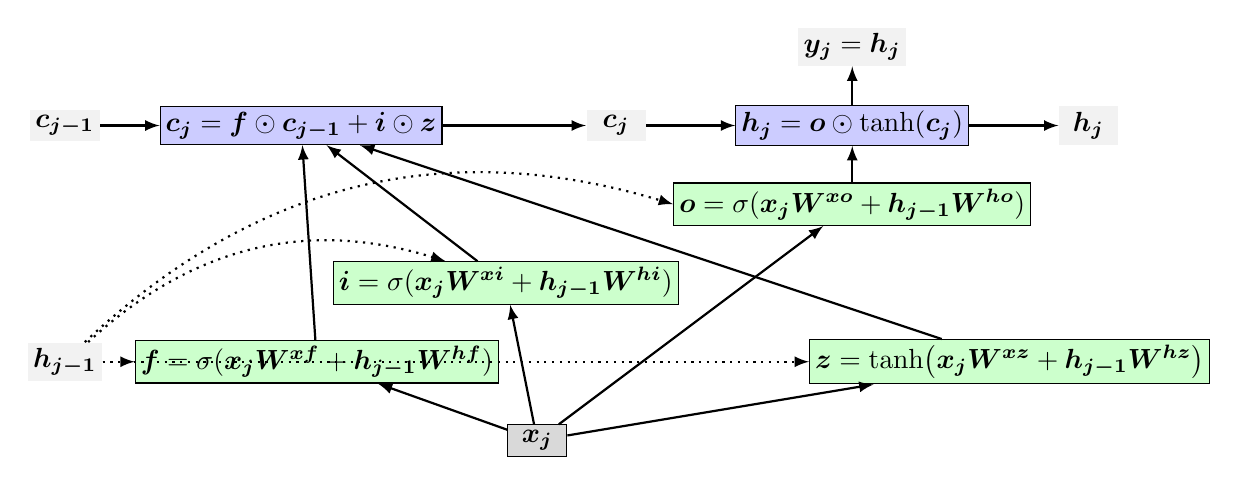
\begin{tikzpicture}	
		
		\onslide<1->{
			\node (c0) [state]{$\bm{c_{j-1}}$};
			\node (h0) [state, below of=c0, yshift=-2cm]{$\bm{h_{j-1}}$};	
			\node (xj) [constant, below of=h0, xshift=6cm] {$\bm{x_j}$};
		}
		
		\onslide<2->{
			\node(z) [param, right of=h0, xshift=11cm] {$\bm{z} = \tanh(\bm{x_j} \bm{W^{xz}} + \bm{h_{j-1} \bm{W^{hz}}} )$};
		}
		
		
		\onslide<3->{
			\node(f) [param, right of=h0, xshift=2.2cm] {$\bm{f} = \sigma(\bm{x_j} \bm{W^{xf}} + \bm{h_{j-1} \bm{W^{hf}}} )$};
		}
		
		\onslide<4->{
			\node(i) [param, right of=h0, xshift=4.6cm, yshift=1cm] {$\bm{i} = \sigma(\bm{x_j} \bm{W^{xi}} + \bm{h_{j-1} \bm{W^{hi}}} )$};
		}
		
		
		\onslide<5->{
			\node(cj) [neuron, right of=c0, xshift=2cm] {$\bm{c_j} = \bm{f} \odot \bm{c_{j-1}} + \bm{i} \odot \bm{z}$};
			
			\node (cjout) [state, right of=cj, xshift=3cm] {$\bm{c_j}$};
		}
		
		\onslide<7->{
			\node(hj) [neuron, right of=cj, xshift=6cm] {$\bm{h_j} = \bm{o} \odot \tanh(\bm{c_j})$};
			
			\node (hjout) [state, right of=hj, xshift=2cm] {$\bm{h_j}$};
		}
		
		\onslide<6->{
			\node(o) [param, below of=hj, xshift=0cm, yshift=0cm] {$\bm{o} = \sigma(\bm{x_j} \bm{W^{xo}} + \bm{h_{j-1} \bm{W^{ho}}} )$};
		}
		\onslide<8->{
			
			\node(yj) [state, above of=hj, yshift=0cm] {$\bm{y_j} = \bm{h_j}$};
		}
		\begin{scope}[thick, black, ->, >=latex]
			
			\onslide<2->{
				\draw(xj) -- (z);
			}
			\onslide<2>{
				\draw [dotted] (h0) -- (z);
			}
			
			\onslide<3->{
				\draw(xj) -- (f);
			}
			\onslide<3>{
				\draw [dotted] (h0) -- (f);
			}
			
			\onslide<4->{
				\draw(xj) -- (i);
			}
			\onslide<4>{
				\draw [dotted] (h0) to [bend left] (i);
			}
			
			\onslide<5->{
				\draw (f) -- (cj);
				\draw (i) -- (cj);
				\draw (z) -- (cj);
				\draw (c0) -- (cj);
				\draw (cj) -- (cjout);
			}
			
			\onslide<6->{
				\draw(xj) -- (o);
			}
			\onslide<6>{
				\draw  [dotted]  (h0) to [bend left] (o.west);
			}
			
			\onslide<7->{
				\draw (o) -- (hj);
				\draw (cjout) -- (hj);
				\draw (hj) -- (hjout);
			}
			
			\onslide<8->{
				\draw (hj) -- (yj);
			}
			
		\end{scope}
		
		
		
	\end{tikzpicture}
\end{figure}

\onslide<2->{
	$\bm{z}$ --- update candidate
}
\end{frame}

\begin{frame}{LSTM parameters and dimensions}

\vspace{-1em}
$$\bm{x_j} \in \mathbb{R}^{d_{in}} \quad
\bm{c_j}, \bm{h_j}, \bm{y_j}, \bm{i}, \bm{f}, \bm{o}, \bm{z} \in \mathbb{R}^{d_h} \quad
\bm{W^{x\star}} \in \mathbb{R}^{d_{in} \times d_{h}} \quad
\bm{W^{h\star}} \in \mathbb{R}^{d_{h} \times d_{h}}$$

$d_h$ --- dimensionality of LSTM (`hidden' layer)

\vspace{-3em}
\begin{figure}
	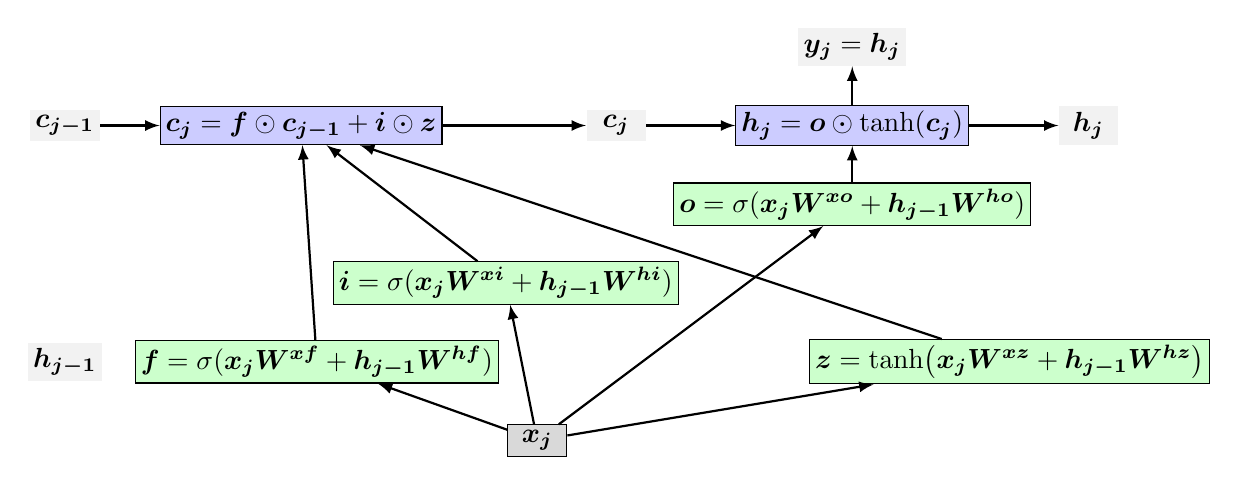
\begin{tikzpicture}	
		
		
		\node (c0) [state]{$\bm{c_{j-1}}$};
		\node (h0) [state, below of=c0, yshift=-2cm]{$\bm{h_{j-1}}$};	
		\node (xj) [constant, below of=h0, xshift=6cm] {$\bm{x_j}$};
		\node(z) [param, right of=h0, xshift=11cm] {$\bm{z} = \tanh(\bm{x_j} \bm{W^{xz}} + \bm{h_{j-1} \bm{W^{hz}}} )$};
		\node(f) [param, right of=h0, xshift=2.2cm] {$\bm{f} = \sigma(\bm{x_j} \bm{W^{xf}} + \bm{h_{j-1} \bm{W^{hf}}} )$};
		\node(i) [param, right of=h0, xshift=4.6cm, yshift=1cm] {$\bm{i} = \sigma(\bm{x_j} \bm{W^{xi}} + \bm{h_{j-1} \bm{W^{hi}}} )$};
		\node(cj) [neuron, right of=c0, xshift=2cm] {$\bm{c_j} = \bm{f} \odot \bm{c_{j-1}} + \bm{i} \odot \bm{z}$};
		
		\node (cjout) [state, right of=cj, xshift=3cm] {$\bm{c_j}$};
		\node(hj) [neuron, right of=cj, xshift=6cm] {$\bm{h_j} = \bm{o} \odot \tanh(\bm{c_j})$};
		
		\node (hjout) [state, right of=hj, xshift=2cm] {$\bm{h_j}$};
		\node(o) [param, below of=hj, xshift=0cm, yshift=0cm] {$\bm{o} = \sigma(\bm{x_j} \bm{W^{xo}} + \bm{h_{j-1} \bm{W^{ho}}} )$};
		
		\node(yj) [state, above of=hj, yshift=0cm] {$\bm{y_j} = \bm{h_j}$};
		
		\begin{scope}[thick, black, ->, >=latex]
			
			
			\draw(xj) -- (z);
			\draw(xj) -- (f);
			\draw(xj) -- (i);
			\draw (f) -- (cj);
			\draw (i) -- (cj);
			\draw (z) -- (cj);
			\draw (c0) -- (cj);
			\draw (cj) -- (cjout);
			\draw(xj) -- (o);
			\draw (o) -- (hj);
			\draw (cjout) -- (hj);
			\draw (hj) -- (hjout);
			\draw (hj) -- (yj);
			
			
		\end{scope}
		
		
		
	\end{tikzpicture}
\end{figure}


\end{frame}


\begin{frame}{LSTM as a `layer'}

\begin{figure}
	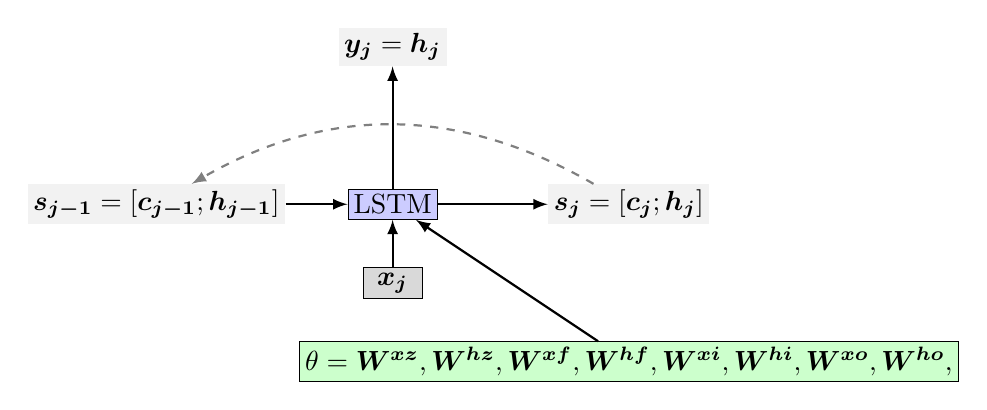
\begin{tikzpicture}	
		%\node (a1) [draw, circle, inner sep=0pt, minimum width=0.75cm, fill=green!20] {$a_1$};
		
		\node (s0) [state]{$\bm{s_{j-1}} = [\bm{c_{j-1}}; \bm{h_{j-1}} ]$};
		
		\node (ro) [neuron, right of=s0, xshift=2cm] {LSTM};
		\node (si) [state, right of=ro, xshift=2cm]{$\bm{s_{j}} = [\bm{c_{j}}; \bm{h_{j}} ]$};
		\node (xi) [constant, below of=ro] {$\bm{x_{j}}$};
		\node(yi) [state, above of=ro, yshift=1cm] {$\bm{y_j} = \bm{h_j}$};
		
		\node (e) [param, below of=si, yshift=-1cm] {$\theta = \bm{W^{xz}}, 
			\bm{W^{hz}},
			\bm{W^{xf}},
			\bm{W^{hf}},
			\bm{W^{xi}},
			\bm{W^{hi}},
			\bm{W^{xo}},
			\bm{W^{ho}},
			$};
		
		
		\begin{scope}[thick, black, ->, >=latex]
			\draw (s0) -- (ro);
			\draw(xi) -- (ro);
			\draw(e) -- (ro);
			\draw(ro) -- (si);
			\draw(ro) -- (yi);
		\end{scope}
		\draw [thick, dashed, gray, ->, >=latex] (si) to [bend right] (s0);
		
	\end{tikzpicture}
\end{figure}

We also ignored bias terms for each gate
\end{frame}

\begin{frame}{LSTM relevance in the Transformer era?}

\begin{quotation}
``How far do we get in language modeling when scaling LSTM to billions of parameters? So far, we can answer: At least as far as current technologies like Transformers or State Space Models. We have enhanced LSTM to xLSTM by exponential gating with memory mixing and a new memory structure.''
\end{quotation}

\begin{tikzpicture}[overlay, remember picture] 
	\node at (current page.north east)[ref] {\fullcite{Beck.et.al.2024.NeurIPS} \par};
\end{tikzpicture}
\end{frame}

\begin{frame}{Take aways}

\begin{itemize}
	\item RNNs for arbitrary long input
	\item Encoding the entire sequence and/or each step
	\item Modeling freedom with bi-directional RNNs
	\item Vanishing gradients in deep nets --- gating mechanism, memory cells
	\item LSTM a particularly powerful RNN
\end{itemize}

\end{frame}



\begin{frame}{License and credits}

	\begin{columns}
		\begin{column}{0.7\textwidth}
			Licensed under Creative Commons Attribution-ShareAlike 4.0 International (CC BY-SA 4.0)
		\end{column}
		\begin{column}{0.2\textwidth}
			\includegraphics[width=0.9\linewidth]{img/cc-by-sa-icon.pdf}
		\end{column}
	\end{columns}
	
	\bigskip
	
	Credits
	
	\begin{scriptsize}
		
		Ivan Habernal
		
		Content from ACL Anthology papers licensed under CC-BY \url{https://www.aclweb.org/anthology}
		
	
	\end{scriptsize}
	
\end{frame}

\appendix


\section{Appendix: Skip-Gram in word2vec}

\begin{frame}{Skip-Gram --- even more relaxed context notion}

\begin{figure}
	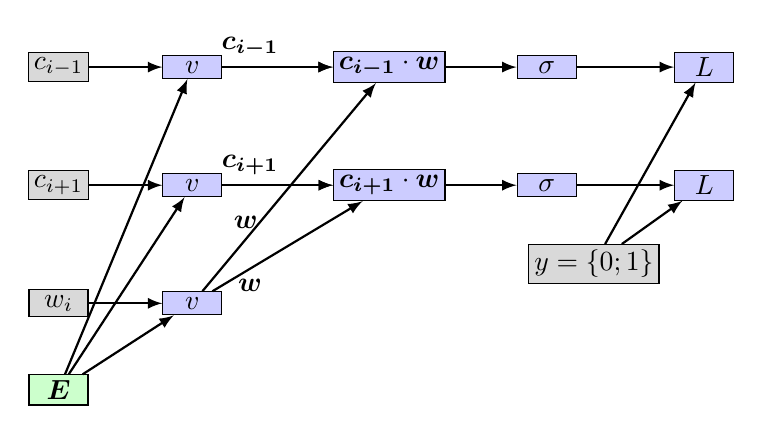
\begin{tikzpicture}	
		%\node (a1) [draw, circle, inner sep=0pt, minimum width=0.75cm, fill=green!20] {$a_1$};
		
		\node (the) [constant] {$c_{i-1}$};
		\node (black) [constant, below of=the, yshift=-0.5cm]{$c_{i+1}$};
		\node (dog) [constant, below of=black, yshift=-0.5cm]{$w_i$};
		\node (e) [param, below of=dog, yshift=-0.1cm] {$\bm{E}$};
		
		\node (lookup1) [neuron, right of=the, xshift=0.7cm] {$v$};
		\node (lookup2) [neuron, below of=lookup1, yshift=-0.5cm] {$v$};
		\node (lookup3) [neuron, below of=lookup2, yshift=-0.5cm] {$v$};			
%		\node (concat) [neuron, right of=lookup1, xshift=0.5cm, yshift=-1cm] {sum};
		
		
		%			\node (x) [constant, right of=concat, xshift=1cm] {$\bm{x}$};
		\node (f11) [neuron, right of=lookup1, xshift=1.5cm] {$\bm{c_{i-1}} \cdot \bm{w}$};
		\node (f12) [neuron, right of=lookup2, xshift=1.5cm] {$\bm{c_{i+1}} \cdot \bm{w}$};
		
		\node (sigma1) [neuron, right of=f11, xshift=1cm] {$\sigma$};
		\node (sigma2) [neuron, right of=f12, xshift=1cm] {$\sigma$};
		
		\node (l1) [neuron, right of=sigma1, xshift=1cm] {$L$};
		\node (l2) [neuron, right of=sigma2, xshift=1cm] {$L$};
		\node (y) [constant, below of=sigma2, xshift=0.6cm] {$y = \{0; 1\}$};
		
		\begin{scope}[thick, black, ->, >=latex]
			\draw (the) -- (lookup1);
			\draw (black) -- (lookup2);
			\draw (dog) -- (lookup3);
			\draw (e) -- (lookup1);
			\draw (e) -- (lookup2);
			\draw (e) -- (lookup3);
			
			\draw (lookup1) -- (f11);
			\draw (lookup2) -- (f12);
			\draw (lookup3) -- (f11) node [near start, above] {$\bm{w}$};
			\draw (lookup3) -- (f12) node [near start, below] {$\bm{w}$};			
			
			\draw (lookup1) -- (f11) node [near start, above] {$\bm{c_{i-1}}$};
			\draw (lookup2) -- (f12) node [near start, above] {$\bm{c_{i+1}}$};
			\draw (f11) -- (sigma1);
			\draw (f12) -- (sigma2);
			\draw (sigma1) -- (l1);
			\draw (sigma2) -- (l2);
			\draw (y) -- (l1);
			\draw (y) -- (l2);
		\end{scope}	
	\end{tikzpicture}
\end{figure}

For $k$-element context $c_{1:k}$, treat as $k$ different independent contexts $(w_i, c_i)$


\end{frame}

\begin{frame}{Choosing the context}

\begin{block}{Sliding window approach --- CBOW}
Auxiliary tasks are created by taking a sequence of $2m + 1$ words
\begin{itemize}
	\item The middle word is the target (focus) word
	\item The $m$ words to each side is the context
\end{itemize}
\end{block}

\begin{block}{Sliding window approach --- Skip-Gram}
$2m$ distinct tasks are created, each pairing the focus word with a different context word
\end{block}	

Skip-gram-based approaches shown to be robust and efficient to train

\end{frame}



\section{FastText embeddings: Sub-word embeddings}

\begin{frame}{FastText embeddings}

Popular word embedding models ignore the morphology of words, by assigning a distinct vector to each word.
\begin{itemize}
\item Limitation, especially for languages with large vocabularies and many rare words
\end{itemize}

\pause

$\to$ Model each word as a bag of character $n$-grams
\begin{itemize}
\item Each character $n$-gram has own embedding
\item Word is represented as a sum of $n$-gram embeddings	
\end{itemize}

\begin{tikzpicture}[overlay, remember picture] 
	\node at (current page.north east)[ref] {\fullcite{Bojanowski.et.al.2017.TACL} \par};
\end{tikzpicture}


\end{frame}

\begin{frame}{FastText embeddings example}
	
Extract all the character $n$-grams for $3 \leq n \leq 6$

\begin{example}
\texttt{eating} $\to$ $G_w = \{$
\texttt{<ea}, \texttt{eat}, \texttt{ati}, \texttt{tin}, \texttt{ing}, \texttt{ng>},
\texttt{<eat}, \texttt{eati}, \texttt{atin}, \texttt{ting}, \texttt{ing>},
\texttt{<eati}, \texttt{eatin}, \texttt{ating}, \texttt{ting>},
\texttt{<eatin}, \texttt{eating}, \texttt{ating>} $\}$
$$
v(\text{eating}) = \sum_{g \in G_w} v(G_w)
$$
\end{example}

Train with skip-gram and negative sampling (same as word2vec)

\begin{tikzpicture}[overlay, remember picture] 
	\node at (current page.north east)[ref] {\fullcite{Bojanowski.et.al.2017.TACL} \par};
\end{tikzpicture}


\end{frame}

\end{document}

